\documentclass{article}
\usepackage[zh]{homework}
\usepackage{tikz}
\usetikzlibrary{arrows.meta}

\config{Algebra-1}{2026 秋季}{2}

\begin{document}

\textbf{我承诺: 本次作业的完成没有使用大语言模型.}

\paragraph{范围} 第三,四讲: 子范畴(subcategory),子群胚(subgroupoid),群(group),自由群(free group)与泛性质(universal property). 共 15 题, 第 15 题为选读/选做.

\paragraph{约定} 以下范畴均假设局部小(locally small), 未加说明的函子均指协变函子(covariant functor). $\mathbf{Set}$ 和 $\mathbf{Grp}$ 分别是集合与函数,群与群同态组成的范畴; 固定一个域 $k$, $\mathbf{Vect}_k$ 是 $k$-向量空间与 $k$-线性映射组成的范畴. $\Hom_{\mathcal C}(X,Y)$ 表示从 $X$ 到 $Y$ 的态射集, $\Aut_{\mathcal C}(X)$ 是其中所有可逆自态射在复合下组成的群, $\operatorname{Map}(A,B)$ 表示集合 $A$ 到集合 $B$ 的全部函数. $U:\mathbf{Grp}\to\mathbf{Set}$ 是取群的底层集合,取群同态的底层函数的遗忘函子. $f\circ g$ 表示先作 $g$ 再作 $f$.

对群 $G$, 以 $1_G$ 记单位元(加法群中记为 $0$), $\langle S\rangle$ 表示包含 $S\subseteq G$ 的最小子群; 特别地, $\langle\varnothing\rangle=\{1_G\}$. $\operatorname{ord}(g)$ 是 $g$ 的阶(order). 对同态 $f:G\to H$, $\ker f=\{g\in G:f(g)=1_H\}$, $\operatorname{im}f=f(G)$. $\Aut(G)$ 是群 $G$ 的所有自同构在复合下组成的群. 记 $\mathbb N_0=\{0,1,2,\ldots\}$; $d\mid n$ 表示整数 $d$ 整除 $n$.

\paragraph{请仔细阅读此定理} 定义群 $\mathbb Z/n\mathbb Z$: 对正整数 $n$, 若 $n\mid(a-b)$, 记 $a\equiv b\pmod n$. 令 $\bar a=\{b\in\mathbb Z:b\equiv a\pmod n\}$, 并定义 $\mathbb Z/n\mathbb Z=\{\bar 0,\bar 1,\ldots,\overline{n-1}\}$, 其加法为 $\bar a+\bar b=\overline{a+b}$. 加法与代表元的选择无关; $\bar 0$ 是单位元, $\overline{-a}$ 是 $\bar a$ 的逆元, 故这是一个含 $n$ 个元素的加法群. 我们也记 $\mathbb Z/n\mathbb Z$ 为 $C_n$. 称其为(阶为 $n$)的循环群.

本作业涉及的群及子群非空; 本题组允许空范畴和空子范畴. 除题面给出的定义或明确允许引用的前题结论外, 请写出证明; 不预设商群理论,Sylow 定理或拓扑知识.

\section*{习题}

\begin{problem}
  设 $G$ 是群, $\mathbf{B}G$ 是对应的单对象群胚, 其唯一对象记为 $*$, 箭头复合由群乘法给出.
  \begin{enumerate}
    \item[(a)] 对子集 $H\subseteq G$, 说明何时 $\{*\}$ 与箭头集 $H$ 构成 $\mathbf{B}G$ 的子范畴(subcategory), 何时构成子群胚(subgroupoid). 用加法下的 $\mathbb N_0\subseteq\mathbb Z$ 给出子范畴不是子群胚的例子.
    \item[(b)] 证明: 对一个子群 $H\leq G$, $\mathbf{B}H\subseteq\mathbf{B}G$ 是满子范畴(full subcategory)当且仅当 $H=G$. 再证明: 群胚的满子范畴一定是子群胚.
    \item[(c)] 对范畴 $\mathcal C$, 其核心群胚 $\mathcal C^\simeq$ 保留所有对象和所有可逆态射. 证明 $\mathcal C^\simeq\subseteq\mathcal C$ 是满子范畴当且仅当 $\mathcal C$ 是群胚.
    \item[(d)] 完整验证群同态 $H\to G$ 与函子 $\mathbf{B}H\to\mathbf{B}G$ 一一对应. 特别说明保持逆元为何由函子条件推出, 而不必另列为条件.
  \end{enumerate}
\end{problem}

\begin{solution}
	\paragraph{(a)} 若对于任意的 $h_1,h_2 \in H$, 均有 $h_1h_2 \in H$, 且 $1_G\in H$, 则对于任意的 $h_1,h_2 \in H \subset \Aut_{\mathbf{B}G}(*)$, 均有 $h_1\circ h_2 \in H$, 并且 $1_{*} \in H$, 此时 $(\{*\},H)$ 构成 $\mathbf{B}G$ 的子范畴; 反过来也可以证明, 若 $(\{*\},H)$ 构成 $\mathbf{B}G$ 的子范畴, 则对于任意的 $h_1,h_2\in H$, 均有 $h_1h_2\in H$, 且 $1_G \in H$.

	若除此之外, 还有对于任意的 $h\in H$, 均有 $h^{-1}\in H$, 则对于任意的 $h\in H\subset \Aut_{\mathbf{B}G}(*)$, 均存在 $h^{-1}\in H$ 使得 $h \circ h^{-1} = h^{-1} \circ h = 1_{*}$, 即 $h$ 是同构, 因而 $(\{*\}, H)$ 构成 $\mathcal{B}G$ 的子群胚; 反过来, 若 $(\{*\}, H)$ 构成 $\mathbf{B}G$ 的子群胚, 则对于任意的 $h\in H$, 均有 $h^{-1}\in H$.

	对于 $\mathbb{N}_0 \subset \mathbb{Z}$, 首先有 $1_{(\mathbb{Z},+)} = 0 \in \mathbb{N}_0$, 并且对于任意的 $a,b\in \mathbb{N}_0$, 均有 $a+b \in \mathbb{N}_0$, 因此 $(\{*\}, \mathbb{Z}_0)$ 给出了 $\mathbf{B}\mathbb{Z}$ 的子范畴; 但是, 对于 $0<a \in \mathbb{N}_0$, $-a \not\in \mathbb{N}_0$, 因此 $\Aut_{\mathbf{B}\mathbb{Z}}(*) \ni a^{-1} \notin \mathbb{N}_0$, 因而 $a$ 在子范畴 $(\{*\}, \mathbb{Z}_0)$ 中不是同构, 因此此子范畴不是子群胚.

	\paragraph{(b)} 注意到
	\[ H=G \Longleftrightarrow \End_{\mathbf{B}H}(\{*\}) = \End_{\mathbf{B}G}(\{*\}) \Longleftrightarrow \mathbf{B}H \subset \mathbf{B}G \text{ 是满子范畴.} \]

	对于任意的一个群胚 $\mathcal{G}$ 及其满子范畴 $\mathcal{H}$, 对于 $\mathcal{H}$ 中的态射 $X \xrightarrow{h} Y$, 由于 $\Hom_{\mathcal{H}}(X,Y) = \Hom_{\mathcal{G}}(X,Y)$, 则 $h^{-1} \in \Hom_{\mathcal{H}}(Y,X)$, 即 $h$ 在子范畴 $\mathcal{H}$ 中也是同构, 因此 $\mathcal{H}$ 是群胚.

	\paragraph{(c)} 注意到
	\[ \begin{array}{cc}
		 & \mathcal{C}^{\cong} \subset \mathcal{C} \text{ 是满子范畴} \\
		\Longleftrightarrow & \forall\, X,Y\in \operatorname{Obj}(\mathcal{C}),\ \Hom_{\mathcal{C}^{\cong}}(X,Y) = \Hom_{\mathcal{C}}(X,Y) \\
		\Longleftrightarrow & \forall\, (X \xrightarrow{f} Y) \in \mathcal{C}, \Hom_{\mathcal{C}^{\cong}}(Y,X) \ni f^{-1} \in \Hom_{\mathcal{C}}(Y,X) \\
		\Longleftrightarrow & \mathcal{C} \text{ 是群胚.}
	\end{array} \]

	\paragraph{(d)} 对于群同态 $f: H \to G$, 构造函子 $\mathbf{B}f: \mathbf{B}H \to \mathbf{B}G$, 满足 $\mathbf{B}f(*_{\mathbf{B}H}) = *_{\mathbf{B}G}$, 并且
	\[ \forall\,h\in H = \Aut_{\mathbf{B}H}(*_{\mathbf{B}H}),\  \mathbf{B}f(h) = f(h) \in G = \Aut_{\mathbf{B}G}(*_{\mathbf{B}G}). \]

	下面来验证 $\mathbf{B}f$ 是一个函子: 对于 $1_{*_{\mathbf{B}H}}$, $\mathbf{B}f(1_{*_{\mathbf{B}H}}) = f(1_H) = 1_g = 1_{*_{\mathbf{B}G}}$; 而对于 $h_1,h_2 \in = \Aut_{\mathbf{B}H}(*_{\mathbf{B}H})$, 有
	\[ \mathbf{B}f(h_1) \circ \mathbf{B}f(h_2) = f(h_1) \circ f(h_2) = f(h_1h_2) = \mathbf{B}f(h_1\circ h_2). \]
	因此 $\mathbf{B}f$ 是一个函子. 

	反过来, 对于一个函子 $\mathbf{B}f: \mathbf{B}H \to \mathbf{B}G$, 定义群同态 $f: H \to G$ 如下: 对于 $h \in H = Aut_{\mathbf{B}H}(*_{\mathbf{B}H})$, 定义 $f(h) = \mathbf{B}f(h) \in = \Aut_{\mathbf{B}G}(*_{\mathbf{B}G}) = G$. 
	
	下面来验证 $f$ 是一个群同态. 对于 $h_1,h_2 \in H$, 有
	\[ f(h_1)f(h_2) = \mathbf{B}f(h_1) \circ \mathbf{B}f(h_2) = \mathbf{B}f(h_1\circ h_2) = f(h_1h_2). \]
	并且, $f(1_H)f(1_H) = f(1_H1_H) = f(1_H)$, 从而 $f(1_H) = 1_G$; 对于 $h\in H$, 有 $f(h)f(h^{-1}) = f(hh^{-1}) = f(1_H) = 1_G$, 因此 $f(h^{-1}) = f(h)^{-1}$.
	因此 $f$ 是一个群同态.
\end{solution}



\begin{problem}
  \begin{enumerate}
    \item[(a)] 设 $\varnothing\neq H\subseteq G$. 证明 $H\leq G$ 当且仅当 $xy^{-1}\in H$ 对所有 $x,y\in H$ 成立.
    \item[(b)] 设 $H\subseteq G$ 有限且非空, 并对乘法封闭. 证明 $H$ 是子群. 给出无限情形中结论不成立的例子.
    \item[(c)] 设 $H,K\leq G$. 证明 $H\cup K$ 是子群当且仅当 $H\subseteq K$ 或 $K\subseteq H$.
    \item[(d)] 设 $f:G\to H$ 是群同态. 证明 $\ker f\leq G$,$\operatorname{im}f\leq H$; 若 $L\leq H$, 证明 $f^{-1}(L)\leq G$.
    \item[(e)] 设 $G=\langle S\rangle$ ($G$ 由 $S$ 生成), $H$ 是任意群, $f_1,f_2:G\to H$ 是群同态. 证明若它们在 $S$ 上相同, 则 $f_1=f_2$.
  \end{enumerate}
\end{problem}

\begin{solution}
	\paragraph{(a)} 必要性是显然的, 下面证明充分性. 取 $x \in H$, 知 $1_G = xx^{-1} \in H$, 即 $1_G \in H$; 对于 $h\in H$, 有 $h^{-1} = 1_G h^{-1} \in H$; 对于 $h_1,h_2\in H$, 由 $h_2^{-1}\in H$ 知 $h_1h_2 = h_1(h_2^{-1})^{-1} \in H$. 因此 $H \le G$.

	\paragraph{(b)} 我们只需要验证 $1_G \in H$, 并且任意的 $h\in H$, 均有 $h^{-1} \in H$. 对于任意的 $h\in H$, 考虑 
	\[\{h^{n}: n \ge 1\} \subset H.\]
	由于 $H \subset G$ 是有限的, 因此存在不同的正整数 $n_1<n_2$, 使得 $h^{n_1} = h^{n_2}$, 即 $h^{n_2-n_1} = 1_G \in H$. 
	并且, 由于 $1_G = h^{n_2-n_1} = hh^{n_2-n_1-1}$, 因此 $h^{n_2-n_1-1} = h^{-1} \in H$.
	因此 $H \le G$.

	另一方面, 考虑乘法群 $(\R_+,\cdot)$. 容易知道 $\Z_+$ 是 $\R_+$ 的非空子集并且对乘法封闭, 但是 $(\Z_+,\cdot)$ 不构成群.

	\paragraph{(c)} 充分性显然, 下面证明必要性. 若 $H\not\subset K$ 且 $K\not\subset H$, 则可以取 $g_1 \in H-K$, $g_2 \in K-H$. 由于 $(H \cup K) \le G$, 因此 $g_1g_2 \in H\cup K$. 不妨设 $g_1g_2 \in H$, 则由 $g_1\in H-K\subset H$ 知 $g_2 \in H$, 但这与 $g_2 \in K-H$ 矛盾.
	
	\paragraph{(d)} 对于 $k_1,k_2 \in\ker f$, 有 $f(k_1/k_2) = f(k_1)/f(k_2) = 1_H/1_H = 1_H$, 因此 $k_1/k_2 \in\ker f$, 这说明 $\ker f \le G$. 

	对于 $h_1=f(g_1)\in \im f$ 与 $h_2 = f(g_2) \in \im f$, 有 $h_1/h_2 = f(g_1) f(g_2^{-1}) = f(g_1/g_2) \in \im f$, 即 $h_1/h_2 \in \im f$, 因此 $\im f \le H$. 

	若 $L \le H$, 取 $g_1,g_2 \in f^{-1}(L)$, 则 $f(g_1),f(g_2) \in L$, 因此 $f(g_1/g_2) = f(g_1)/f(g_2) \in L$, 从而 $g_1/g_2 \in f^{-1}(L)$, 因此 $f^{-1}(L) \le H$.

	\paragraph{(e)} 对于任意的 $g\in G = \langle S \rangle$, 存在非负整数 $n$, 整数 $k_1,\dots,k_n$ 以及 $s_1,\dots,s_n \in S$, 使得 $g = s_1^{k_1}s_2^{k_2} \dots s_n^{k_n}$. 则
	\[ f_1(g) = \prod_{i=1}^{n}f_1(s_i)^{k_i} = \prod_{i=1}^{n}f_2(s_i)^{k_i} = f_2(g)
	\implies f_1 = f_2. \]
\end{solution}



\begin{problem}
  \begin{enumerate}
    \item[(a)] 证明 $\mathbb Z$ 的每个子群都唯一地写成 $d\mathbb Z:=\langle d\rangle$ 的形式, 其中 $d\geq0$. 对整数 $m,n$, 证明 $\langle m,n\rangle=\gcd(m,n)\mathbb Z$, 其中约定 $\gcd(0,0)=0$.
    \item[(b)] 设群 $G$ 中的元素 $g$ 满足其阶有限且记其阶为 $n$. (不用 Lagrange 定理,)证明 $g^r=1$ 当且仅当 $n\mid r$, 并推出
      \[
        \operatorname{ord}(g^r)=\frac{n}{\gcd(n,r)}\qquad(r\in\mathbb Z).
      \]
    \item[(c)] 在循环群 $C_{24}$ 中, 计算 $\langle\bar4\rangle$,$\langle\bar6\rangle$,它们的交以及 $\langle\bar4,\bar6\rangle$ 的全部元素. 取 $g=\bar1$, $r=4,6$, 检验第 (b) 问的阶公式.
  \end{enumerate}
\end{problem}

\begin{solution}
	\paragraph{(a)} 考虑 $\Z$ 的任意一个子群 $G$. 若 $G = \{0\}$, 取 $d = 0$ 即可. 否则, 记
	\[ d = \min\{\abs{g}>0: g\in G\} \subset \Z_0. \]
	(由于上面的集合是自然数的子集, 由最小自然数原理知 $d$ 存在.) 则对于任意的整数 $n \in \Z$, 均有 $nd \in G$, 因此 $d\Z \subset G$. 而对于任意的 $g\in G$, 若 $g\notin d\Z$, 则考虑带余除法: $g = qd+r$, 其中 $q\in\Z$, $r\in\{1,2,\dots,d-1\}$. 则 $r = g-qd \in G$, 并且 $q$ 非零, $\abs{r}<d$, 这与 $d$ 的定义矛盾.

	下面来证明 $\bracket{m,n} = \gcd(m,n)\Z$. 由初等数论中的 Bezout 定理, 知 $\gcd(m,n)\in \bracket{m,n}$, 因此 $\gcd(m,n)\Z \subset \bracket{m,n}$; 另一方面, 对于任意的 $x \in \bracket{m,n}$, 存在 $a,b\in\Z$ 使得 $x = am+bn$, 而由 $\gcd(m,n) | m$ 与 $\gcd(m,n) | n$ 知 $\gcd(m,n) | x$, 即 $x \in \gcd(m,n)\Z$. 结合上面两个结果, 知 $\bracket{m,n} = \gcd(m,n)\Z$.

	\paragraph{(b)} 考虑群同态 $f: \Z \to G,\ n \mapsto g^n$. 则 $\ker f \le \Z$, 由 (a) 中的结论, 存在正整数 $n'$, 使得 $\ker f = n'\Z$. 则
	\[ n = \ord(g) = |\im f| = \#\{f(0), f(1), \dots, f(n'-1)\} = n'. \]
	(不难验证 $f(0), f(1), \dots,f(n'-1)$ 两两不同. )即 $n'=n$. 故
	\[ g^r = 1_G \Longleftrightarrow r \in \ker f \Longleftrightarrow n \mid r. \]

	下面来计算 $\ord(g^r)$, 由 $\ord(g) = n \mid \operatorname{lcm}(n,r) = r (n/gcd(n,r))$ 知 $g^{r(n/gcd(n,r))} = 1_G$, 因此 $\ord(g^r) \mid n/gcd(n,r)$; 由 $g^{r \ord(g^r)} = 1_G$ 知 $n \mid r \ord(g^r)$, 即
	\[ \left. \frac{n}{\gcd(n,r)}\,\right|\, \frac{r}{\gcd(n,r)} \ord(g^r).  \]
	结合 $\gcd(n/\gcd(n,r), r/\gcd(n,r)) = 1$, 知 $n/\gcd(n,r) \mid \ord(g^r)$. 

	因此 $\ord(g^r) = n/\gcd(n,r)$.

	\paragraph{(c)} 在 $C_{24}$ 中, $\bracket{\bar{4}} = \{\bar{0}, \bar{4}, \bar{8}, \bar{12}, \bar{16}, \bar{20}\}$, $\bracket{\bar{6}} = \{\bar{0}, \bar{6}, \bar{12}, \bar{18}\}$, $\bracket{\bar{4}} \cap \bracket{\bar{6}} = \{\bar{0}, \bar{12}\}$. 并且, 
	\[ \bracket{\bar{4}, \bar{6}} = \{\bar{0}, \bar{2}, \bar{4}, \dots \bar{22}\}. \]

	取 $g = \bar{1}$, 则 $r = 4$ 或 $6$ 时, 
	\[ \ord(\bar{4}) = \frac{24}{\gcd(24,4)} = 6, \quad \ord(\bar{6}) = \frac{24}{\gcd(24,6)} = 4. \]
\end{solution}



\begin{problem}
  对正整数 $n$, 对称群(symmetric group) $S_n$ 的元素是集合 $\{1,\ldots,n\}$ 到自身的全部双射(bijections), 称为置换(permutations). 群运算是函数复合: $\sigma\tau$ 表示先作用 $\tau$, 再作用 $\sigma$; 单位元是恒等映射, 逆元是逆函数.

  对两两不同的 $i_1,\ldots,i_r\in\{1,\ldots,n\}$ ($2\leq r\leq n$), 循环记号(cycle notation) $(i_1\ i_2\ \cdots\ i_r)$ 表示把 $i_1$ 送到 $i_2$,$i_2$ 送到 $i_3$,依次把 $i_r$ 送回 $i_1$, 并固定其余元素的置换. 长度为二的循环称为换位(transposition). 例如, 在 $S_4$ 中,
  \[
    (1\ 2\ 3\ 4):\quad 1\mapsto2,\quad 2\mapsto3,\quad 3\mapsto4,\quad 4\mapsto1.
  \]
  \begin{enumerate}
    \item[(a)] 在 $S_4$ 中令 $\sigma=(1\ 2\ 3\ 4)$,$\tau=(1\ 3)$. 计算 $\sigma\tau$,$\tau\sigma$,$\sigma\tau\sigma^{-1}$, 并求这些置换的阶.
    \item[(b)] 证明对任意 $\rho\in S_n$
      \[
        \rho(i\ j)\rho^{-1}=(\rho(i)\ \rho(j)).
      \]
      再证明 $S_n$ 由相邻换位 $(1\ 2),(2\ 3),\ldots,(n-1\ n)$ 生成($n\geq2$).
  \end{enumerate}
\end{problem}

\begin{solution}
	\paragraph{(a)} 计算得
	\[ \sigma\tau = (1\ 4)(2\ 3), \quad 
	\tau\sigma = (1\ 2)(3\ 4),\quad 
	\sigma\tau\sigma^{-1} = (2\ 4) \]
	这些元素的阶均为 $2$.

	\paragraph{(b)} 直接计算得到
	\begin{align*}
		\rho \circ  (i\ j) \circ \rho^{-1}(x)
		&= \rho \circ (i\ j) (\rho^{-1}(x)) 
		= \rho \left( \begin{cases}
			j, & \rho^{-1}(x) = i \\
			i, & \rho^{-1}(x) = j \\
			\rho^{-1}(x), & \text{其余情况}
		\end{cases} \right)
		= \begin{cases}
			\rho(j), & x = \rho(i) \\
			\rho(i), & x = \rho(j) \\
			x, & \text{其余情况}
		\end{cases}
		=(\rho(i)\ \rho(j))(x).
	\end{align*}

	再来证明 $S_n = \bracket{(i\ i+1): 1\le i\le n-1}$. 记后者为 $S$, 只需要证明 $S_n = S$. 根据前面的结论, 对于 $1\le i \le n-2$, 有
	\[ (i+1\ i+2)(i\ i+1)(i+1\ i+2) = (i\ i+2) \in S. \]
	若已经知道, 对某一个 $2\le k\le n-2$, 有 $(i\ i+k)\in S$ 对任意的 $1\le i\le n-k$ 成立, 则对于任意的 $1\le i\le n-k-1$,
	\[ (i+k\ i+k+1)(i\ i+k)(i+k\ i+k+1) = (i\ i+k+1) \in S. \]
	根据数学归纳法, 知对于任意的 $1\le i<j\le n$, 均有 $(i\ j)\in S$. 因此, 对于任意的轮换 $(i_1\ i_2\ \dots\ i_k)$ (其中 $i_1, \dots, i_k$ 两两不同), 有
	\[ (i_1\ i_2\ \dots\ i_k) = (i_1\ i_2)\dots(i_{k-2}\ i_{k-1})(i_{k-1}\ i_k) \in S. \]
	而所有的置换都可以分解为不相交的轮换的乘积, 因此所有的置换都属于 $S$, 因此 $S=S_{n}$.
\end{solution}



\begin{problem}
  {\heiti 内自同构群}(\textbf{inner automorphism group}). 定义
  \[
    Z(G)=\{z\in G:zg=gz\text{ 对所有 }g\in G\},\qquad
    \text{对任意 }g\in G,\ \text{定义 }\phi_g(x)=gxg^{-1}:G\to G.
  \]
  我们在课上已经证明上述构造定义了映射:
  \[
    \Phi:G\longrightarrow\Aut(G),\qquad g\longmapsto\phi_g,
  \]
  并令 $\operatorname{Inn}(G)=\{\phi_g:g\in G\}$.
  \begin{enumerate}
    \item[(a)] 证明 $Z(G)\leq G$. 验证每个 $\phi_g$ 都是群 $G$ 的自同构, 并验证
      \[
        \phi_g\circ\phi_h=\phi_{gh},\qquad \phi_g^{-1}=\phi_{g^{-1}}.
      \]
      从而证明 $\Phi:G\to\Aut(G)$ 是群同态, $\operatorname{Inn}(G)\leq\Aut(G)$ (称 $\operatorname{Inn}(G)$ 为 $G$ 的内自同构群), 且 $\ker\Phi=Z(G)$.
    \item[(b)] 对任意 $\alpha\in\Aut(G)$, 证明
      \[
        \alpha\phi_g\alpha^{-1}=\phi_{\alpha(g)}.
      \]
      推出 $\operatorname{Inn}(G)$ 在所有 $\Aut(G)$ 中的共轭下不变. (这样的子群称为正规子群(normal subgroup).)
    \item[(c)] 计算 $\Aut(\mathbb Z)$,$\operatorname{Inn}(\mathbb Z)$,$\Aut(C_8)$ 和 $\operatorname{Inn}(C_8)$, 并给出一个不是内自同构的自同构.
    \item[(d)] 证明 $Z(S_3)=\{1\}$, 并证明 $S_3$ 的每个自同构都是内自同构.
  \end{enumerate}
\end{problem}

\begin{solution}
	\paragraph{(a)} 先来验证 $\phi_g$ 是 $G$ 的自同构. 对于任意的 $g_1,g_2\in G$, 均有
	\[ \phi_g(g_1)\phi_g(g_2) = g g_1 g^{-1} g g_2 g^{-1} = g (g_1g_2) g^{-1} = \phi_g(g_1g_2). \]
	因此 $\phi_g$ 是自同态. 并且对于 $g'\in G$, $\phi_g(g^{-1}g'g) = gg^{-1}g'gg^{-1} = g'$, 因此 $\phi_g^{-1}(g')$ 存在, 因此 $\phi_g$ 是满同态. 并且, 对于 $g_1, g_2 \in G$, 若 $\phi_g(g_1) = \phi_g(g_2)$, 则 $gg_1g^{-1} = gg_2g^{-1}$, 即 $g_1 = g_2$, 因此 $\phi_g$ 也是单同态, 从而 $\phi_g\in\Aut(G)$. 

	下面来验证 $\Phi$ 是群同态. 对于任意的 $g,h\in G$, 有
	\[ \phi_g \circ \phi_h(x) = g(hxh^{-1})g^{-1} = (gh) x (gh)^{-1} = \phi_{gh}. \]
	因此 $\Phi$ 是群同态. 
	
	注意到 $Z(G) = \ker \Phi$, 因此 $Z(G) \le G$. 并且, 由于 $\Inn(G) = \im \Phi$, 因此 $\Inn(G) \le \Aut(G)$.

	\paragraph{(b)} 对于任意的 $x\in G$,
	\[ (\alpha \circ \phi_g \circ \alpha^{-1})(x)
	= \alpha(g(\alpha^{-1}(x)g^{-1}))
	=\alpha(g) \alpha(\alpha^{-1}(x)) \alpha(g^{-1})
	=\phi_{\alpha(g)}(x). \]
	因此 $\alpha \phi_g \alpha^{-1} = \phi_{\alpha(g)}$. 由此知 $\Inn(G) \lhd \Aut(G)$.

	\paragraph{(c)} 由于 $\Z = \bracket{1}$, 知 $\Z$ 的群同构由 $1$ 的像唯一确定. 而对于 $\phi \in \Aut(\Z)$, 由于 $\phi$ 为满射, 则 $\phi(1) \in \{\pm 1\}$, 故 $\Aut(\Z) \cong \Z_2$. (我们记 $\Z_n := \Z/n\Z$. )

	由于 $\Z$ 交换, 因此所有的共轭都是恒等映射, 因此 $\Inn(\Z) \cong \{1\}$.

	取 $\Z_8$ 的生成元 $1$ 以及 $\phi\in \Aut(\Z_8)$. 由于 $\ord(1) = 8$, 则 $\ord(\phi(1)) = 8$, 因此只能有 $\phi(1) \in \{1,3,5,7\}$. 记 $\phi_i \in \Aut(\Z_8)$ 是满足 $\phi_i(1) = i$ ($i \in \{1,3,5,7\}$) 的自同构. 计算得 $\phi_3^2 = \phi_5^2 = \phi_7^2 = \phi_1$, 并且 $\phi_3 \phi_5 = \phi_7$, 因此 $\Aut(\Z_8) \cong \Z_2 \times \Z_2$.

	由于 $\Z_8$ 交换, 因此所有的共轭都是恒等映射, 因此 $\Inn(\Z_8) \cong \{1\}$.

	事实上, $\Aut(\Z_8)$ 中的任何非恒等自同构都不是内自同构.

	\paragraph{(d)} 考虑 $S_3$ 的一个自同构 $\phi \in \Aut(S_3)$. 由于 $S_3 = \bracket{(1\ 2), (2\ 3)}$, $(1\ 2)$ 和 $(2\ 3)$ 的像唯一决定了 $\phi$. 由此可以列出所有的自同构 (每一行代表一个自同构): 
	\[ \begin{array}{cc|cccc}
		(1\ 2) & (1\ 3) & (1) & (2\ 3) & (1\ 2\ 3) & (1\ 3\ 2) \\ \hline
		(1\ 2) & (1\ 3) & (1) & (2\ 3) & (1\ 2\ 3) & (1\ 3\ 2) \\
		(1\ 2) & (2\ 3) & (1) & (1\ 3) & (1\ 3\ 2) & (1\ 2\ 3) \\
		(1\ 3) & (1\ 2) & (1) & (2\ 3) & (1\ 3\ 2) & (1\ 2\ 3) \\
		(1\ 3) & (2\ 3) & (1) & (1\ 2) & (1\ 2\ 3) & (1\ 3\ 2) \\
		(2\ 3) & (1\ 2) & (1) & (1\ 3) & (1\ 2\ 3) & (1\ 3\ 2) \\
		(2\ 3) & (1\ 3) & (1) & (1\ 2) & (1\ 3\ 2) & (1\ 2\ 3)
	\end{array} \]
	观察可知, 这 $6$ 个自同构两两不同, 且 $\Aut(S_3) \cong S_3$. 

	现在来证明 $Z(S_3) = \{1\}$. 事实上, $(1\ 2)$, $(2\ 3)$, $(1\ 3)$ 两两互不交换, 并且均与 $(1\ 2\ 3)$ 或 $(1\ 3\ 2)$ 不交换, 因此 $Z(S_3) = \{1\}$. 因此 $\ker \Phi = \{1\}$. 再结合 $\abs{\Aut(S_3)} = \abs{S_3} = 6$, 知 $\Phi$ 是满同态.
\end{solution}



\begin{problem}
  {\heiti 初对象, 终对象}(\textbf{initial and terminal objects}). 范畴 $\mathcal C$ 中, 一个元素 $0$ (只是记号)是初对象(initial object), 指对每个 $X$, $\Hom_{\mathcal C}(0,X)$ 恰有一个元素; $1$ (只是记号)是终对象(terminal object, 也称 final object), 指 $\Hom_{\mathcal C}(X,1)$ 恰有一个元素. 兼具两种性质的对象称为零对象(zero object).
  \begin{enumerate}
    \item[(a)] 证明任意两个初对象之间存在唯一同构; 终对象也一样. 证明初对象,终对象的自同态都只有恒等态射.
    \item[(b)] 先证明: 对任意两个群 $A,B$, 至少存在一个群同态 $A\to B$. 再写出两个不同的群同态 $\mathbb Z\to\mathbb Z$, 并据此说明 $\mathbb Z$ 既不是 $\mathbf{Grp}$ 的初对象, 也不是终对象. 最后解释: 如果在初对象和终对象的定义中把"恰有一个态射"改成"至少存在一个态射", 那么每个群都会满足这两个削弱后的条件.
    \item[(c)] 分别确定 $\mathbf{Set}$, $\mathbf{Grp}$, $\mathbf{Vect}_k$ 中的初对象与终对象, 并直接验证泛性质. 对固定集合 $T$, 记 $\mathcal P(T)$ 为 $T$ 的幂集, 考虑其作为偏序集对应的范畴 $\mathcal C_{(\mathcal P(T),\subseteq)}$, 确定其初对象与终对象.
    \item[(d)] 固定 $S\subseteq G$. 令 $\mathcal S_{S,G}$ 的对象为包含 $S$ 的子群, 且仅在 $H\subseteq K$ 时有一支箭头 $H\to K$. 考虑其作为偏序集对应的范畴, 证明在这个范畴里 $\langle S\rangle$ 是初对象, $G$ 是终对象.
    \item[(e)] 把 $\mathbf{B}G$ 本身当作范畴. 证明它有初对象当且仅当 $G=\{1_G\}$, 终对象也一样. 再分别指出 $\mathbf{B}G$ 和 $\mathbf{Grp}$ 的对象及态射, 以说明平凡群为何是 $\mathbf{Grp}$ 的零对象.
  \end{enumerate}
\end{problem}

\begin{solution}
	\paragraph{(a)} 根据定义, $\End_{\mathcal{C}}(0) = \Hom_\mathcal{C}(0,0)$ 只有一个元素, 因而只能是 $\id_{0}^{\mathcal{C}}$. 同理, $\End_{\mathcal{C}}(1) = \{\id_{1}^{\mathcal{C}}\}.$. 
	
	下面证明两个初对象之间存在唯一同构. 考虑两个不同的处对象 $0,0'$. 由定义, 存在唯一的态射 $f \in \Hom_\mathcal{C}(0,0')$ 与 $g \in \Hom_\mathcal{C}(0',0)$. 则 $g \circ f \in \End_{\mathcal{C}}(0)$, 故 $g \circ f = \id_0^{\mathcal{C}}$. 同理, $f \circ g = \id_{0'}^{\mathcal{C}}$. 因此 $f$ 与 $g$ 均为同构, 故 $0 \cong 0'$.

	同理, 若 $\mathcal{C}$ 有两个终对象 $1, 1'$, 则同样有 $1 \cong 1'$. 

	\paragraph{(b)} 构造映射 $f: A \to B$, 对任意的 $a \in A$, 令 $f(a) = 1_B$. 显然 $f$ 是群同态, 因此 $f \in \Hom_{\mathbf{Grp}}(A,B)$. 

	不难知道, 映射 $n \mapsto n$ 与 $n \mapsto 0$ 均为 $\Z$ 与 $\Z$ 之间的群同态, 因此 $\Z$ 既不是 $\mathbf{Grp}$ 的初对象也不是终对象. 

	事实上, 对于任意的群 $A,B$, 根据上面的讨论, $\Hom_{\mathbf{Grp}}(A,B)$ 均非空, 因而每个群都满足: 对于任意的群 $G$, $\Hom_{\mathbf{Grp}}(A,G)$ 与 $\Hom_{\mathbf{Grp}}(G,A)$ 均非空.

	\paragraph{(c)} $\mathbf{Set}$ 的初对象是 $\varnothing$, 终对象是任意单元集 $\{1\}$. 对于任意的集合 $S$, $\Hom_{\mathbf{Set}}(\varnothing, S)$ 包含且仅包含一个空映射, $\Hom_{\mathbf{Set}}(S,\{1\})$ 包含且仅包含映射 $s \mapsto 1$. 

	$\mathbf{Grp}$ 的初对象和终对象均为平凡群 $\{1\}$. 对于任意的群 $G$, $\Hom_{\mathbf{Grp}}(\{1\}, G)$ 包含且仅包含一个群同态 $1 \mapsto 1_G$, $\Hom_{\mathbf{Grp}}(G, \{1\})$ 包含且仅包含一个群同态 $g \mapsto 1$. 

	$\mathbf{Vect}_k$ 的初对象和终对象均为平凡线性空间 $\{0\}$. 对于任意的线性空间 $V$, $\Hom_{\mathbf{Vect}_k}(\{0\}, V)$ 包含且仅包含一个线性映射 $0 \mapsto 0_V$, $\Hom_{\mathbf{Vect}_k	}(V, \{0\})$ 包含且仅包含一个线性映射 $v \mapsto 0$.

	$\mathcal{C}_{(\mathcal{P}(T), \subset)}$ 的初对象为 $\varnothing$, 终对象为 $T$. 这是因为, 初对象 $0$ 满足 $0 \subset S$ 对于任意的 $S \subset T$ 成立, 特别地也对 $S = \varnothing$ 成立, 因此 $0 = \varnothing$; 终对象 $1$ 满足 $S \subset 1$ 对任意的 $S \subset T$ 成立, 特别地也对 $S = T$ 成立, 因此 $1 = T$. 

	\paragraph{(d)} 对于任意的群 $H \in \Obj(\mathcal{S}_{S,G})$, 根据定义, $S \subset H$, 因此 $\bracket{S} \le H$, 即 $\Hom_{\mathcal{S}(S,G)}(\bracket{S}, H)$ 恰好有一个元素, 因此 $\bracket{S}$ 是初对象. 对于任意的 $H \in \Obj(\mathcal{S}_{S,G})$, 根据定义, $H \le G$, 因此 $\Hom_{\mathcal{S}(S,G)}(H,G)$ 恰好有一个元素, 因此 $G$ 是终对象.

	\paragraph{(e)} 注意到
	\[ \mathbf{B}G \text{ 有终对象} 
	\Longleftrightarrow \#(\End_{\mathbf{B}G}(*_{\mathbf{B}G})) = 1
	\Longleftrightarrow |G| = 1
	\Longleftrightarrow G = \{1\}. \]
	对初对象也同理.

	$\mathbf{B}G$ 的对象只有 $*_{\mathbf{B}G}$, 态射只有 $*_{\mathbf{B}G}$ 的恒等态射; $\mathbf{Grp}$ 的对象为所有的群, 态射为所有的群同态. 根据 (c) 中的结论, 平凡群是 $\mathbf{Grp}$ 的零对象.
\end{solution}



\begin{problem}
  {\heiti 集合的纤维积及其泛性质}(\textbf{fiber products of sets}). 给定集合映射 $f:X\to Z$, $g:Y\to Z$, 定义纤维积(fiber product, 也称 pullback)
  \[
    X\times_Z Y=\{(x,y)\in X\times Y:f(x)=g(y)\},
  \]
  并定义投影 $\pi_X(x,y)=x$, $\pi_Y(x,y)=y$, 所以 $f\circ\pi_X=g\circ\pi_Y$.
  \begin{enumerate}
    \item[(a)] 证明如下泛性质: 对任意集合 $T$ 及映射 $a:T\to X$, $b:T\to Y$, 若 $f\circ a=g\circ b$, 则存在唯一映射 $u:T\to X\times_Z Y$ 使
      \[
        \pi_X\circ u=a,\qquad \pi_Y\circ u=b.
      \]
      必须显式写出 $u$, 并分别证明其良定义性和唯一性.
    \item[(b)] 定义辅助范畴 $\mathcal P(f,g)$: 对象为满足 $f\circ a=g\circ b$ 的三元组 $(T,a:T\to X,b:T\to Y)$; 态射 $h:(T,a,b)\to(T',a',b')$ 满足 $a'\circ h=a$, $b'\circ h=b$. 验证它是范畴, 并证明 $(X\times_ZY,\pi_X,\pi_Y)$ 是终对象. 由此证明任何两个满足上述泛性质的对象, 都存在唯一的,与两个投影相容的同构.
    \item[(c)] 取 $Z=\{0,1\}$, $X=\{1,2,3\}$, $Y=\{a,b,c\}$, 令
      \[
        f(1)=f(2)=0,\qquad f(3)=1,\qquad g(a)=0,\qquad g(b)=g(c)=1.
      \]
      列出 $X\times_ZY$ 的全部元素, 以及两个投影的值.
    \item[(d)] 当 $Z$ 是单点集时, 说明纤维积如何变为通常的 Cartesian 积.
    \item[(e)] 若 $X,Y\subseteq Z$ 且 $f,g$ 都是包含映射, 验证此时有 $X\times_ZY\cong X\cap Y$ 的典范双射, 并说明此时的投影如何理解.
  \end{enumerate}
\end{problem}

\begin{solution}
	\paragraph{(a)} 构造 $u: T \to X \times_Z Y$, 使得对任意的 $t \in T$, 
	\[ u(t) = (a(t), b(t)). \]
	
	先来证明 $u(t) \in X \times_Z Y$, 即 $u$ 是良定义的. 这是因为, 由 $f \circ a = g \circ b$, 知 $f(a(t)) = g(b(t))$, 因此 $u(t) = (a(t), b(t)) \in X \times_Z Y$. 

	再来证明 $u$ 满足条件. 注意到
	\[ \pi_X \circ u(t) = \pi_X((a(t),b(t))) = a(t), \quad
	\pi_Y \circ u(t) = \pi_Y((a(t),b(t))) = b(t). \]
	因此 $u$ 满足条件.

	再来证明唯一性. 设还存在 $u'$ 满足条件. 我们来证明 $u = u'$. 事实上, 根据投影的定义, 对于任意的 $t \in T$, 有
	\[ u(t) = (\pi_X(u(t)), \pi_Y(u(t))) = (a(t), b(t))
	 = (\pi_X(u'(t)), \pi_Y(u'(t))) = u'(t). \]

	\paragraph{(b)} 先来验证 $\mathcal{P}(f,g)$ 构成范畴. 
	\begin{enumerate}[label=(\arabic*)]
		\item 对于一个对象 $(T,a,b)$, 映射 $h := \id_T^{\mathbf{Set}}$ 满足 $a \circ h = a$, $b \circ h = b$, 因此 $\id_{(T,a,b)}^{\mathcal{P}(f,g)} = \id_T^{\mathbf{Set}}$. 
		\item 对于 $\mathcal{P}(f,g)$ 中的两个态射 $(T,a,b) \xrightarrow{h} (T',a',b') \xrightarrow{h'} (T'',a'',b'')$, 将 $h,h'$ 看做 $\Hom_{\mathbf{Set}}(T,T')$ 与 $\Hom_{\mathbf{Set}}(T',T'')$ 中的映射进行符合, 得到 $h' \circ h$. 由于
		\[ a' \circ h = a, \quad a'' \circ h' = a' \implies a'' \circ (h' \circ h) = a. \]
		同理, $b'' \circ (h' \circ h) = b$. 因此 $h' \circ h$ 是 $\mathcal{P}(f,g)$ 中 $(T,a,b)$ 到 $(T'',a'',b'')$ 的态射.
		\item 由于 $\mathcal{P}(f,g)$ 中态射的复合可以看做映射的复合, 因此结合律满足.
		\item 由于 $\mathcal{P}(f,g)$ 中的恒等态射是集合的恒等映射, 因此恒等态射公理满足.
	\end{enumerate}

	而根据 (a) 中的结论, $(X \times_Z Y, \pi_X, \pi_Y)$ 是 $\mathcal{P}(f,g)$ 的终对象. 而根据上一题的结论, 任何满足上述泛性质的对象, 都存在唯一的同构.

	\paragraph{(c)} $X \times_Z Y = \{(1,a), (2,a), (3,b), (3,c)\}$. 两个投影的值如下: 
	\[ \begin{array}{c|cccc}
		x & (1,a) & (2,a) & (3,b) & (3,c) \\ \hline 
		\pi_X(x) & 1 & 2 & 3 & 3 \\
		\pi_Y(x) & a & a & b & c
	\end{array} \]

	\paragraph{(d)} 若 $Z$ 是单点集, 则对于任意的 $x\in X$ 与 $y\in Y$, $f(x)$ 与 $g(y)$ 均等于 $Z$ 中的唯一元素, 因此 $f(x) = g(y)$. 从而 $X \times_Z Y = X \times Y$.

	\paragraph{(e)} 由于 $f,g$ 均为嵌入映射, 因此 $f(x) = x$, $g(y) = y$. 因此, 对于 $(x,y) \in X \times_Z Y$, 由 $f(x) = g(y)$ 知 $x=y \in X \cap Y$. 反过来, 对于 $x=y \in X \cap Y$, 有 $f(x) = g(y)$, 因此 $(x,y) \in X \times_Z Y$. 因此在上述意义下, $X \times_Z Y$ 与 $X \cap Y$ 之间存在典范双射.
	
	此时, 投影 $\pi_X$ 可以理解为 $X \cap Y$ 到 $X$ 的嵌入映射, $\pi_Y$ 同理.
\end{solution}



\begin{problem}
  {\heiti 有限循环群的判别法}(\textbf{a criterion for finite cyclic groups}). 对正整数 $d$, 定义 Euler 函数(Euler's totient function)
  \[
    \varphi(d)=\#\{1\leq r\leq d:\gcd(r,d)=1\},\qquad\varphi(1)=1.
  \]
  \begin{enumerate}
    \item[(a)] 利用第 3 题, 证明阶为 $d$ 的循环群恰有 $\varphi(d)$ 个生成元. 再按元素的阶对 $C_n$ 分类, 证明
      \[
        \sum_{d\mid n}\varphi(d)=n.
      \]
      其中求和遍历 $n$ 的所有正因数.
    \item[(b)] 设 $G$ 是基数为 $n$ 的有限群, 不预设 $G$ 是交换群. 证明: $G$ 是循环群, 当且仅当对每个正因数 $d\mid n$, 都有
      \[
        \#\{x\in G:x^d=1_G\}\leq d.
      \]
      证明中若使用了"元素的阶整除群的阶", 请先给出其初等证明: 可考察集合 $h\langle x\rangle$ 如何把 $G$ 分成等大的不交部分.
    \item[(c)] 应用第 (b) 问, 证明任意域 $k$ 的乘法群 $k^\times=k\setminus\{0\}$ 中的有限子群都是循环群. 本问可使用: 域上的非零 $d$ 次多项式至多有 $d$ 个根.
  \end{enumerate}
  提示: 纪念 Jean-Pierre Serre 百岁: 想找线索, 可以翻他的 \emph{A Course in Arithmetic} 第 I 章 §1.2 正文. 本判别法似乎不是 Serre 最初提出的, 但具体出处未查到. Serre 在书中用此结果证明任意域中的元根(primitive root)的存在性.
\end{problem}

\begin{solution}
	\paragraph{(a)} 由于 $x$ 为 $\Z_d$ 的生成元当且仅当 $\ord(x) = d$, 因此 $\Z_d$ 的生成元的数量为
	\begin{align*}
		\# \{x \in \Z_d: \ord(x) = d\}
		&= \# \left\{x \in \Z_d: \frac{d}{\gcd (x,d)}=d\right\}
		= \# \left\{ x\in \Z_d: \gcd (x,d) = 1 \right\}
		= \varphi(d).
	\end{align*}

	根据问题 3(b) 的结论, 对于 $\Z_n$ 的一个元素 $m$, 其阶整除 $n$, 并且 $\ord(m) = n/\gcd (m,n)$. 因此
	\begin{align*}
		n 
		&= \sum_{d|n}^{} \#\{m \in \Z_n: \ord(m) = d\}
		= \sum_{d|n}^{} \#\{m \in \Z_n: (m,n) = n/d\} \\
		&= \sum_{d|n}^{} \varphi \left( \frac{n}{n/d} \right)
		= \sum_{d|n}^{} \varphi(d).
	\end{align*}

	\paragraph{(b)} 先来证明``元素的阶整除群的阶''. 
	设 $x \in G$. 令 $r = \ord(x)$, 则 $H := \langle x\rangle = \{1_G,x,\ldots,x^{r-1}\}$, $|H| = r$.

	对于任意的 $h \in G$, 令 $hH = \{ha:a \in H\}$. 映射 $H \to hH$, $a \mapsto ha$ 是双射, 其逆映射为 $b \mapsto h^{-1}b$, 因此 $|hH| = r$.

	再来证明任意两个这样的集合或者相等, 或者不交. 若 $hH \cap kH \neq \varnothing$, 则存在 $a,b \in H$ 使 $ha = kb$, 从而 $h = kba^{-1}$. 由于 $H$ 是子群, 对任意的 $c \in H$, 有 $hc = k(ba^{-1}c) \in kH$, 因此 $hH \subset kH$. 同理 $kH \subset hH$, 因此 $hH = kH$.

	最后, 每个 $h \in G$ 都属于 $hH$, 因此这些集合覆盖 $G$. 将其中不同的集合记为 $h_1H,\ldots,h_tH$, 则它们将 $G$ 分成 $t$ 个两两不交的部分, 每个部分都有 $r$ 个元素. 因此 $|G| = tr$, 即 $\ord(x) \mid |G|$.

	回到原题. 对 $n$ 的一个因子 $d$, 若存在以 $d$ 为阶的元素, 记为 $g$, 则 $\bracket{g} = \{1_G, g, g^{2}, \dots, g^{d-1}\}$. 则 $\bracket{g}$ 中的所有元素的 $d$ 次方均为 $1_G$, 结合题目条件便知
	\[ \{x \in G: x^{d} = 1_G\} = \bracket{g}. \]

	再来考察阶恰好为 $d$ 的元素. 这些元素必须在 $\bracket{g}$ 中, 而由 $\ord(g^{k}) = d/\gcd(k,d)$ 知
	\[ \{x \in G: \ord(x) = d\} = \{g^{k}: 0\le k<d, \gcd(k,d) = 1\}. \]

	因此, 若存在以 $d$ 为阶的元素, 则恰好有 $\varphi(d)$ 个以 $d$ 为阶的元素. 结合 $n = \sum_{d|n}^{}\varphi(d)$, 知对于任意的 $d|n$, 均恰好有 $\varphi(d)$ 个以 $d$ 为阶的元素. 取 $d = n$, 知存在阶为 $n$ 的元素, 因此 $G$ 为循环群.

	\paragraph{(c)} 由于多项式 $x^d - 1$ 在 $k$ 中至多有 $d$ 个根, 因此 $k^\times$ 中至多有 $d$ 个元素满足 $x^{d} = 1$. 直接使用 (b) 中的结论便证明了命题.
\end{solution}



\begin{problem}
  {\heiti 约化字}(\textbf{reduced words}){\heiti 的存在性与唯一性}. 本题及随后三题依次构造自由群, 验证群公理, 证明泛性质, 并与初对象定义对接. 本题只能使用普通字的连接和约化规则; 群结构将在下一题建立.

  令 $I$ 为集合, $I^\pm=I\times\{+1,-1\}$; 把 $(i,+1)$ 记为 $i$, 把 $(i,-1)$ 记为 $\bar i$. 这里 $i$ 与 $\bar i$ 是两个不同的形式字母. 对任意字母 $a\in I^\pm$, $\bar a$ 表示交换其标记, 故 $\bar{\bar a}=a$. 本题中的横线只作用于形式字母; 群元素的逆将在下一题用上标 $-1$ 表示.

  令 $W(I)$ 为 $I^\pm$ 上的全部有限字(word), 包括空字 $\varepsilon$; 字的前后连接记为 $uv$. 定义一步约化为删除字中的一对相邻字母 $a\bar a$. 一个字中没有这类相邻对子的字称为约化字(reduced word).
  \begin{enumerate}
    \item[(a)] 证明对任意字连续进行约化, 这一过程最终停止.
    \item[(b)] 若同一个字可以分别约化一步得到 $u,v$, 分析两次消去的位置: 相同,互不相交,或重叠. 证明存在某个字 $z$, 使 $u,v$ 都可以通过若干次消去到达 $z$. 重叠时必须明确分析长度为三的字 $a\bar a a$.
    \item[(c)] 对原字长度作强归纳, 证明每个字最终得到的约化字唯一, 记为 $\operatorname{red}(w)$. 这里主要是唯一性证明.
    \item[(d)] 对任意字 $u,v$, 证明
      \[
        \operatorname{red}(\operatorname{red}(u)v)=\operatorname{red}(uv)
        =\operatorname{red}(u\operatorname{red}(v)).
      \]
      并计算 $\operatorname{red}(xy\bar y\bar x)$ 与 $\operatorname{red}(xy\bar x x\bar y)$ ($x,y\in I$ 且 $x\neq y$).
  \end{enumerate}
\end{problem}

\begin{solution}
	\paragraph{(a)} 字的长度有限, 而每次约化操作会使得字的长度减 $2$, 因此约化操作最终停止.

	\paragraph{(b)} 假设约化位置为 $\{i,i+1\}$ 的两个字母得到 $u$, 约化位置为 $\{j,j+1\}$ 的两个字母得到 $v$. 不妨设 $i<j$. (若 $i=j$, 两次约化操作时等价的. )

	若 $j = i+1$, 则两次约化操作的位置有重叠. 此时, 第 $i$、第 $i+2$ 个字母均为第 $i+1$ 个字母的``逆'', 因此这三个字母必须形如 $a \bar{a} a$. 不难验证, 无论是约化前两个字母, 还是约化后两个字母, 得到的结果均为 $a$. 因此 $u=v$.

	若 $j > i+1$, 则两次约化操作是交换的, 因此对 $u$ 约化 $\{j-2,j-1\}$ 处的字母, 与对 $v$ 约化 $\{i,i+1\}$ 处的字母, 得到的结果是相同的.

	\paragraph{(c)} 对于字 $w$, 将它的长度记为 $l(w) \in \Z_+$. 我们来通过对 $l\ge 1$ 证明: 所有满足 $l(w) = l$ 的字 $w$ 的约化均唯一. 

	命题对 $l = 0, 1, 2$ 显然成立. 假设命题对不大于 $l-1$ 的所有正整数成立, 其中 $l \ge 3$, 接下来证明命题对于 $l$ 也成立. 对于满足 $l(w) = l$ 的字 $w$, 设它有 $k$ 种约化的方式, 并且按每一种方式约化后得到的字分别为 $w_1, w_2, \dots, w_k$. 若 $k=0$ 则命题已经成立; 若 $k=1$, 则对 $w_1$ 使用归纳假设, 知命题成立. 下面考虑 $k\ge 2$ 的情况.

	由归纳假设, 知每一个 $w_i$ 最终得到的约化字唯一. 而根据 (b) 中的结论, 对于任意的 $1 \le i < j \le k$, 都可以对 $w_i$ 和 $w_j$ 进行至多一步操作, 得到一个字 $w_{ij}$. 由于 $w_{ij}$ 最后得到的约化字唯一, $w_i$ 与 $w_j$ 最后得到的约化字也唯一, 因此三者相等. 也就是说, 对于任意的 $1 \le i < j \le k$, $w_i$ 与 $w_j$ 最终得到的唯一约化字相同. 因此无论如何约化 $w$, 最后都会得到唯一的约化字. 

	\paragraph{(d)} 由于两个等式的证明是类似的, 我们只证明前一个. 对 $l(uv)$ 归纳. $l(uv) = 0, 1, 2$ 时, 命题显然成立. 假设对任意满足 $l(uv)< l$ 的字 $u,v$, 命题均成立, 其中 $l \ge 3$. 

	若 $\operatorname{red}(u) = u$, 则命题显然成立, 因此可以假设 $u$ 不是既约的. 设 $u$ 可以通过一步约化变成 $u'$, 则 $\operatorname{red}(u) = \operatorname{red}(u')$, 并且注意到 $u'v$ 可以看做 $uv$ 经过一步约化得来, 因此 $\operatorname{red}(uv) = \operatorname{red}(u'v)$. 而由于 $l(u'v)<l(uv)$, 根据归纳假设, 有 $\operatorname{red}(u'v) = \operatorname{red}(\operatorname{red}(u')v) = \operatorname{red}(\operatorname{red}(u) v)$, 因此 $\operatorname{red}(\operatorname{red}(u)v) = \operatorname{red}(uv)$.

	计算: $\operatorname{red}(xy\bar{y}\bar{x}) = \varepsilon$; $\operatorname{red}(xy\bar{x}x\bar{y}) = x$.
\end{solution}

\begin{problem}
  {\heiti 字群的两种模型与单生成元自由群}(\textbf{word groups and the free group on one generator}). 记 $F(I)$ 为第 9 题中全部约化字组成的集合.
  \begin{enumerate}
    \item[(a)] 对 $u,v\in F(I)$ 定义 $u*v=\operatorname{red}(uv)$. 用第 9 题的结论证明 $*$ 满足结合律, 且空字 $\varepsilon$ 是单位元. 若 $u=a_1\cdots a_n$ 是约化字, 令 $v=\bar a_n\cdots\bar a_1$; 证明 $v$ 也约化, 且 $u*v=v*u=\varepsilon$. 由此证明 $(F(I),*)$ 是群, 并得到群元素的取逆公式
      \[
        u^{-1}=\bar a_n\cdots\bar a_1.
      \]
      当 $u=\varepsilon$ 时, 右边也按空字理解.
    \item[(b)] 证明 $\eta_I:I\to F(I)$, $i\mapsto i$ 是单射, 且其像生成刚刚构造出的群. 说明每个生成字母都不是单位元.
    \item[(c)] 在 $W(I)$ 上定义 $u\sim v$: 可以通过有限次插入或删除相邻逆字母对, 把 $u$ 变成 $v$. 证明这是与连接相容的等价关系, 且
      \[
        u\sim v\quad\Longleftrightarrow\quad\operatorname{red}(u)=\operatorname{red}(v).
      \]
      记 $W(I)/{\sim}$ 为所有等价类组成的集合. 证明 $G_I^{\mathrm{word}}=W(I)/{\sim}$ 在 $[u][v]=[uv]$ 下成为群, 写出 $[a_1\cdots a_n]$ 的逆, 并证明映射 $G_I^{\mathrm{word}}\to F(I)$,$[w]\mapsto\operatorname{red}(w)$ 是群同构.
    \item[(d)] 令 $I=\{x\}$, 先用形式字母 $x,\bar x$ 列出全部约化字, 再证明构造出的群中每个元素都唯一写成 $x^m$ ($m\in\mathbb Z$), 其中 $x^0=\varepsilon$, 负指数按第 (a) 问的群逆解释. 验证以下乘法公式, 并证明所给映射 $\theta$ 是群同构:
      \[
        x^m*x^n=x^{m+n},\qquad
        \theta:F(\{x\})\longrightarrow(\mathbb Z,+),\qquad x^m\longmapsto m.
      \]
      写出 $\theta$ 的逆映射, 并说明为何 $x$ 具有无限阶. 另计算 $F(\varnothing)$. 本问必须从约化字构造出发, 不得只引用"单生成元自由群是 $\mathbb Z$".
    \item[(e)] 在 $F(\{x\})$ 中计算 $x^4*(x^{-1})^7$ 和 $(x^{-3})^{-1}$. 证明 $x^m\mapsto\bar m$ 定义满同态 $F(\{x\})\to C_5$, 并求其核. 说明 $C_5$ 可由一个元素生成, 并分别说明 $C_5$ 与 $F(\{x\})$ 中非单位元的阶.
  \end{enumerate}
\end{problem}

\begin{solution}
	\paragraph{(a)} 先证明结合律. 根据第 9 题的结论, 
	\[ (u * v) * w = \operatorname{red}(\operatorname{red}(uv)w)
	=\operatorname{red}(uvw) = \operatorname{red}(u\operatorname{red}(vw))
	=u * (v * w). \]

	根据空字 $\varepsilon$ 的定义, 对于任意的字 $w$, 均有 $w\varepsilon = \varepsilon w = w$, 因此 $w*\varepsilon = \varepsilon*w = w$. 

	若 $u = a_1a_2\dots a_n$ 是约化字, 则对于任意的 $1\le i \le n-1$, 均有 $a_i \neq \bar{a}_{i+1}$, 则 $\bar{a}_{i+1} \neq \bar{\bar{a}_{i}}$, 故 $u^{-1} := \bar{a}_n\bar{a}_{n-1} \dots \bar{a}_1	$ 是约化字. 直接的计算表明 $u * u^{-1} = u^{-1} * u = \varepsilon$. 

	因此, $(F(I), *)$ 是群.

	\paragraph{(b)} 由于对于每一个 $i \in I$, 字 $i$ 均为约化的, 并且 $I$ 中的字母两两不同, 因此 $\eta_I$ 是单射. $F(I)$ 中的每一个词都是有限长的, 因此可以用有限多个 $I^{\pm}$ 中的元素连接得到, 因此 $F(I) = \bracket{\eta_I(I)}$. 每个 $\eta_I(i)$ 都不等于 $\varepsilon$, 因此每个生成字母都不是单位元.

	\paragraph{(c)} 若 $u_1 \sim u_2$, 且 $v_1 \sim v_2$, 则对于单词 $u_1v_1$, 在 $u_1$ 内部操作为 $u_2$, 再在 $v_1$ 内部操作为 $v_2$, 知可以通过有限次的操作将 $u_1v_1$ 操作为 $u_2v_2$, 因此 $u_1v_1 \sim u_2v_2$. 

	接下来证明 $u \sim v \Longleftrightarrow \operatorname{red}(u) = \operatorname{red}(v)$. 对于必要性, 事实上, 根据等价的定义, 我们只需要证明: 若 $u$ 可以通过删去一对相邻逆字母变为 $v$, 则 $\operatorname{red}(u) = \operatorname{red}(v)$, 而这由 $\operatorname{red}(u)$ 的唯一性保证成立. 而对于充分性, 若 $\operatorname{red}(u) = \operatorname{red}(v)$, 则根据 ``$ \sim $'' 的定义, 有 $u \sim \operatorname{red}(u) = \operatorname{red}(v) \sim v$.

	接下来验证 $G_I^{\mathrm{word}}$ 构成群. 事实上, 对于一个等价类 $[u]$ 中的任意单词 $u' \in [u]$, 均有 $\operatorname{red}(u') = \operatorname{red}(u)$, 因此每一个等价类 $[u]$ 都可以唯一地对应到一个既约字 $\operatorname{red}(u) \in F(I)$. 反过来, 对于任意的 $u\in F(I)$, 都可以唯一地对应到一个等价类 $[u] \in W(I)/\sim$. 并且, 容易验证, 对于 $u,v \in F(I)$, $[u][v] = [uv] = [u * v]$. 因此, $(F(I),*) \cong (W(I)/\sim, [\cdot][\cdot])$. 由于 $(F(I), *)$ 是群, 因此 $G_I^{\mathrm{word}} = W(I)/\sim$ 也构成群, 并且 $[w] \mapsto \operatorname{red}(w)$ 是同构.

	根据上述同构, $[a_1a_2\dots a_n]^{-1} = [\bar{a}_{n}\bar{a}_{n-1}\dots \bar{a}_1]$.

	\paragraph{(d)} 由于 $I$ 中只有一个字母, 因此如果一个字中同时出现了 $x$ 和 $\bar{x}$, 那么必然有至少一对 $x$ 和 $\bar{x}$ 相邻, 因此不是既约的. 所以用 $\{x, \bar{x}\}$ 列出的所有既约字只可能是连续的若干个 $x$ 或 $\bar{x}$. 

	而连续的 $n$ 个 $x$ 等于 $x^{n}$, 连续的 $n$ 个 $\bar{x}$ 等于 $x^{-n}$, $\varepsilon$ 等于 $x^0$, 因此 $F(I) = \{x^n: n \in \Z\}$. 

	根据 ``$*$'' 的定义, 
	\[ x^m * x^n = \operatorname{red}\left(\underbrace{xx\dots x}\limits_{m} \underbrace{xx\dots x}\limits_{n}\right) = x^{m+n}. \]
	再根据同态的定义, 知 $\theta$ 是群同态.

	由于任意多个 $x$ 排在一起组成的字都是既约的, 因此 $x$ 具有无限阶. 

	当 $I = \varnothing$ 时, $F(I)$ 中只有空字 $\varepsilon$ 一个元素, 因此 $(F(\varnothing), *) \cong \{1\}$. 

	\paragraph{(e)} $x^4 * (x^{-1})^7 = x^{-3}$, $(x^{-3})^{-1} = x^{3}$. 

	事实上, 取 $\Z$ 到 $\Z_5$ 的群同态 $f: n \mapsto \bar{n} \mod 5$. 则群同态 $x^{m} \mapsto \bar{m} \mod 5$ 可以写为 $f \circ \theta$, 其中 $\theta$ 的含义与 (d) 中相同. 而 $f$ 和 $\theta$ 均为满同态, 因此不难验证 $f \circ \theta$ 也是满同态. $\ker (f \circ \theta) = \bracket{x^5}$.

	$\Z_5$ 是循环群, 当然可以由一个元素生成. 由于 $5$ 为素数, 因此 $\Z_5$ 中任何非单位元的阶均为 $5$; 而 $F(\{x\})$ 中的任何非单位元的阶均为无穷.
\end{solution}



\begin{problem}
  {\heiti 自由群的泛性质与生成子群}(\textbf{free groups and generated subgroups}). 设 $H$ 是任意群, $\varphi:I\to U(H)$ 是任意集合映射. 定义形式字母的取值映射 $\varphi^\pm:I^\pm\to U(H)$: 对 $i\in I$, 规定
  \[
    \varphi^\pm(i)=\varphi(i),\qquad
    \varphi^\pm(\bar i)=\varphi(i)^{-1}.
  \]
  这里 $\bar i$ 是形式字母, $\varphi(i)^{-1}$ 是 $H$ 中的群逆.
  \begin{enumerate}
    \item[(a)] 定义普通字在 $H$ 中的取值
      \[
        E_\varphi(a_1\cdots a_n)
        =\varphi^\pm(a_1)\cdots\varphi^\pm(a_n),\qquad
        E_\varphi(\varepsilon)=1_H.
      \]
      证明每次消去都保持取值, 所以 $E_\varphi(\operatorname{red}(w))=E_\varphi(w)$.
    \item[(b)] 证明取值给出唯一群同态 $\widetilde\varphi:F(I)\to H$, 满足 $U(\widetilde\varphi)\circ\eta_I=\varphi$. 从而完整证明典范双射
      \[
        \Hom_{\mathbf{Grp}}(F(I),H)\cong\operatorname{Map}(I,U(H)).
      \]
    \item[(c)] 给定 $S\subseteq G$, 令 $f_{\mathrm{can}}:F(S)\to G$ 是包含映射 $S\hookrightarrow U(G)$ 的唯一延拓. 用两种方法证明 $\operatorname{im}f_{\mathrm{can}}=\langle S\rangle$: 一种使用字的取值; 另一种只使用自由群泛性质及 $\langle S\rangle$ 的最小性. 明确写出经过 $\langle S\rangle$ 的分解, 以及用于比较两个同态的唯一性.
    \item[(d)] 推出 $f_{\mathrm{can}}$ 满射当且仅当 $S$ 生成 $G$. 分别描述 $S=\varnothing$ 和 $S=\{1_G\}$ 时的 $F(S)$ 与 $f_{\mathrm{can}}$. 后一种情形, 记 $s=\eta_S(1_G)\in F(S)$; 求 $s$ 和 $f_{\mathrm{can}}(s)$ 的阶.
  \end{enumerate}
\end{problem}

\begin{solution}
	\paragraph{(a)} 对于一对相邻的逆字母 $x\bar{x}$ ($x \in I$), 有 $\varphi^{\pm}(x)\varphi^\pm(\bar{x}) = \varphi(x) \varphi (x) ^{-1} = 1_H$. 同理 $\varphi^\pm(\bar{x}) \varphi^\pm(x) = 1_H$. 因此每一次消去都不会改变取值.

	\paragraph{(b)} 一方面, 若给定了映射 $\varphi: I \to U(H)$, 定义群同态 $\tilde{\varphi}: F(I) \to H$ 如下: 对于 $w \in F(I)$, 取 $\tilde{\varphi}(w) = E_\varphi(w)$. 不难验证 $\tilde{\varphi}$ 是群同态. 则对于任意的 $i\in I$, $U(\tilde{\varphi}) \circ \eta_I(i) = U(\tilde{\varphi})(i) = \varphi(i)$, 因此 $U(\tilde{\varphi}) \circ \eta_I = \varphi$. 

	另一方面, 若给定了群同态 $\tilde{\varphi}: F(I) \to H$, 则定义 $\varphi = U(\tilde{\varphi}) \circ \eta_I$, 知 $\varphi \in \Hom_{\mathbf{Set}}(I,U(H))$.

	若给定了两个群同态 $\tilde{\varphi}_{1,2}: F(I) \to H$, 均满足 $U(\tilde{\varphi}_{1,2}) \circ \eta_I = \varphi$, 我们来证明 $\tilde{\varphi}_1 = \tilde{\varphi}_2$. 事实上, 对于任意的 $i \in I$, 均有 $\tilde{\varphi}_1(i) = \varphi(i) = \tilde{\varphi}_2(i)$ (我们在这里将 $\eta_I(i)$ 看做 $i$). 对于 $w = i_1^{\delta_1}\dots i_n^{\delta_n} \in F(I)$ ($i_j \in I	$, $\delta_j \in \{\pm 1\}$), 有
	\[ \tilde{\varphi}_1(w) 
	= \tilde{\varphi}_1(i_1^{\delta_1}*\dots * i_n^{\delta_n}) 
	=\tilde{\varphi}_1(i_1)^{\delta_1} \dots \tilde{\varphi}_1(i_n)^{\delta_n}
	=\tilde{\varphi}_2(i_1)^{\delta_1} \dots \tilde{\varphi}_2(i_n)^{\delta_n}
	= \tilde{\varphi}_2(i_1^{\delta_1}*\dots * i_n^{\delta_n})
	=\tilde{\varphi}_2(w). \]
	
	因此我们证明了 $\Hom_{\mathbf{Grp}}(F(I), H) \cong \Hom_{\mathbf{Set}}(I, U(H))$.

	\paragraph{(c)} 先用第一种方法证明. 一方面, 对于 $x \in \bracket{S}$, 存在 $s_1, \dots, s_n \in S$ 与 $\delta_1, \dots, \delta_n \in \{\pm 1\}$, 使得 $x = s_1^{\delta_1}\dots s_n^{\delta_n}$ 且 $w := s_1^{\delta_1}\dots s_n^{\delta_n}$ 为 $S$ 上的既约字 (此处将 $s_i^{-1}$ 看做字母 $s_i$ 的形式逆). 由于 $w \in F(S)$, 并且 $x = f_{\mathrm{can}}(w)$, 故 $x \in \im f_{\mathrm{can}}$. 因此 $\bracket{S} \subset \im f_{\mathrm{can}}$.

	另一方面, 对于 $x \in \im f_{\mathrm{can}}$, 存在 $s_1 \dots s_n \in F(S)$, 使得 $x = f_{\mathrm{can}}(s_1\dots s_n)$. 而由于 $f_{\mathrm{can}}\Big|_{S} = \id_S$, 知 $f_{\mathrm{can}}(s_1 \dots s_n) = s_1 \dots s_n \in \bracket{S}$. 因此 $\im f_{\mathrm{can}} \subset \bracket{S}$. 两方面结合即得到两者相等.

	再使用第二种方法证明. 取出两个嵌入映射: $i': S \hookrightarrow \bracket{S}$ 与 $j: \bracket{S} \hookrightarrow H$. 记 $i = j \circ i'$, 则 $i: S \hookrightarrow H$ 也是嵌入映射.

	由 $F(S)$ 的泛性质, 存在唯一的群同态 $f'_{\mathrm{can}}: F(S) \to \bracket{S}$, 使得 $i' = f'_{\mathrm{can}} \circ \eta_I$. 而根据 $f_{\mathrm{can}}$ 的定义, $i = f_{\mathrm{can}} \circ \eta_I$. 

	注意到 
	\[ (j \circ f'_{\mathrm{can}}) \circ \eta_I
	= j \circ (f'_{\mathrm{can}} \circ \eta_I)
	= j \circ i'
	=i, \]
	因此 $i = (j \circ f'_{\mathrm{can}}) \circ \eta_I$. 与上面的结论 $i = f_{\mathrm{can}} \circ \eta_I$ 对比, 结合泛性质, 知 $j \circ f'_{\mathrm{can}} = f_{\mathrm{can}}$. 

	因此, $\im f_{\mathrm{can}} = \im (j \circ f'_{\mathrm{can}}) \subset \im j = \bracket{S}$. 

	另一方面, $S = \im i = \im (f_{\mathrm{can}} \circ \eta_I) \subset \im f_{\mathrm{can}}$. 而 $\im f_{\mathrm{can}} \le H$, 因此根据 $\bracket{S}$ 的定义, 有 $\bracket{S} \subset \im f_{\mathrm{can}}$. 

	综上, $\im f_{\mathrm{can}} = \bracket{S}$.

	% AI 使用声明: 下图由 AI 根据用户提供的手绘图重绘为 TikZ.
	\begin{figure}[H]
	  \centering
	  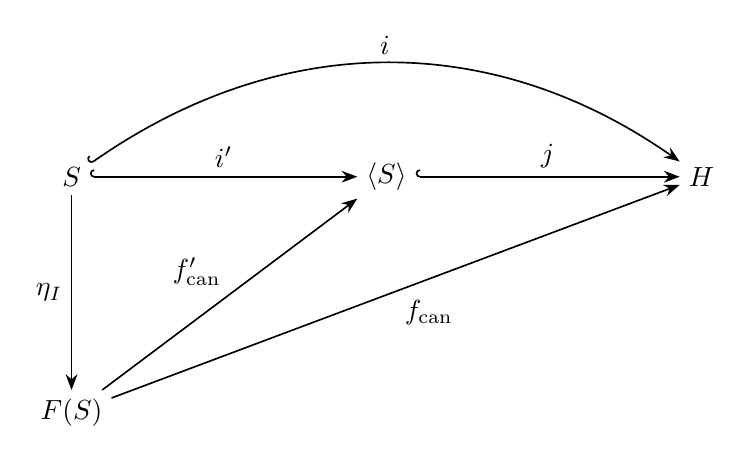
\begin{tikzpicture}[line width=0.6pt, >={Stealth},
	    every node/.style={inner sep=3pt}]
	    \node (S) at (0,0) {$S$};
	    \node (generated) at (4,0) {$\langle S\rangle$};
	    \node (G) at (8,0) {$H$};
	    \node (free) at (0,-3) {$F(S)$};
	    \draw[{Hooks[right]}-{Stealth}] (S) -- node[above] {$i'$} (generated);
	    \draw[{Hooks[right]}-{Stealth}] (generated) -- node[above] {$j$} (G);
	    \draw[{Hooks[right]}-{Stealth}] (S) to[out=35,in=145]
	      node[above] {$i$} (G);
	    \draw[->] (S) -- node[left] {$\eta_I$} (free);
	    \draw[->] (free) -- node[above left] {$f'_{\mathrm{can}}$} (generated);
	    \draw[->] (free) -- node[below right] {$f_{\mathrm{can}}$} (G);
	  \end{tikzpicture}
	\end{figure}

	\paragraph{(d)} $f_{\mathrm{can}}$ 满射 $\Longleftrightarrow$ $\im f_{\mathrm{can}} = G$ $\Longleftrightarrow$ $\bracket{S} = G$ $\Longleftrightarrow$ $S$ 生成 $G$. 
	
	当 $S = \varnothing$ 时, $F(S) = \{1_{F(S)}\}$, $f_{\mathrm{can}}$ 是平凡群同态; 当 $S = \{1_G\}$ 的时候, $F(S) \cong \Z$, 而 $f_{\mathrm{can}}$ 是像为 $\{1_{G}\}$ 的平凡群同态.

	设 $s = \eta_I(1_G) \in F(S)$, 则 $f_{\mathrm{can}}(s) = 1_G$. $s$ 的阶为无穷, 而 $f_{\mathrm{can}}(s) = 1_G$ 的阶为 $1$.
\end{solution}


\begin{problem}
  {\heiti 验证课上定义与参考教材的初对象定义等价}(\textbf{free objects as initial objects}). 给定函子 $U:\mathcal C\to\mathbf{Set}$ 和集合 $I$. 定义范畴 $\mathcal F_U^I$ (也记 $I\downarrow U$): 对象为 $(A,j)$, 其中 $A\in\mathcal C$, $j:I\to U(A)$ 是任意集合映射; 态射 $h:(A,j)\to(B,k)$ 是 $\mathcal C$ 中满足 $U(h)\circ j=k$ 的态射.

  映射 $j$ 可以不是单射, 其像也可以不生成 $A$.
  \begin{enumerate}
    \item[(a)] 验证该定义给出一个范畴, 并证明以下两种条件等价:
      \begin{enumerate}
        \item[(i)] $(F,\eta)$ 是 $\mathcal F_U^I$ 的初对象;
        \item[(ii)] 对每个 $A\in\mathcal C$, 映射
          \[
            \Hom_{\mathcal C}(F,A)\longrightarrow\operatorname{Map}(I,U(A)),
            \qquad h\longmapsto U(h)\circ\eta
          \]
          是双射.
      \end{enumerate}
    \item[(b)] 应用于 $U:\mathbf{Grp}\to\mathbf{Set}$, 证明第 10 题的约化字群与第 11 题的生成映射组成 $\mathcal F_U^I$ 的初对象. 因此它与按教材中"初对象"方式定义的自由群存在唯一的, 保持生成映射的同构. 必须写出两个方向的同态, 并用唯一性验证它们互逆.
    \item[(c)] 证明当 $I\neq\varnothing$ 时, $F(I)$ 本身不是 $\mathbf{Grp}$ 的初对象. 以 $I=\{x\}$ 为例, 比较 $x\mapsto x^{-1}$ 作为底层群自同构与作为 $\mathcal F_U^I$ 中态射的区别.
    \item[(d)] (选做)思考此时这样定义的自由对象是否一定满足 $\eta$ 是单射? (Hint: 令 $\mathcal C$ 只含平凡群及其恒等态射, $U$ 取底层集合, 分析 $|I|\geq2$ 的情形. 另一方面, 仅利用泛性质证明对于 $\mathbf{Grp}\to\mathbf{Set}$, 自由群的生成映射必单射.)
  \end{enumerate}
  提示: 最后一句可以对两个不同生成元, 选择一个到二阶群 $C_2$ 的函数把它们分开.
\end{problem}

\begin{solution}
	\paragraph{(a)} 我们来验证 $\mathcal{F}_U^I$ 是一个范畴. 
	\begin{enumerate}[label=(\arabic*)]
		\item $\mathcal{F}_U^I$ 中的恒等态射为 $\id_{(A,j)}^{\mathcal{F}_U^I} = \id_A^{\mathcal{C}}$.
		\item 对于 $\mathcal{F}_U^I$ 中的两个态射 $(A,j) \xrightarrow{f} (B,k) \xrightarrow{g} (C,l)$, 定义 $f$ 与 $g$ 在 $\mathcal{F}_U^I$ 中的复合即为在 $\mathcal{C}$ 中的复合. 则根据定义, 
		 \[ U(g \circ f) \circ j = U(g) \circ (U(f) \circ j)
		 =U(g) \circ k = l. \]
		 因此, $g \circ f$ 确实是 $(A,j)$ 到 $(C,l)$ 的态射, 此复合是良定义的.
		 \item 由于 $\mathcal{F}_U^I$ 中态射的复合可以看做 $\mathcal{C}$ 中的态射的复合, 因此单位态射公理和结合公理均成立.
	\end{enumerate}

	下面来验证 (i) 与 (ii) 等价. 记 (ii) 中的映射为 $\Phi$, 即 $\Phi(h) = U(h) \circ \eta$.

	``(i) $\implies$ (ii)'': 对于每一个映射 $j \in \Hom_{\mathbf{Set}}(I, U(A))$, $(A,j)$ 为 $\mathcal{F}_{U}^I$ 中的一个对象. 由于 $(F,\eta)$ 为初对象, 因此存在\textit{唯一}的态射 $h: (F,\eta) \to (A,j)$. 将 $h$ 看做 $\mathcal{C}$ 中的态射, 即知 $h$ 是 $\Hom_{\mathcal{C}}(F,A)$	 中\textit{唯一}满足 $U(h) \circ \eta = j$ 的态射. 因此 $\Phi$ 既是单射又是满射, 因此是双射.

	``(ii) $\implies$ (i)'': 对于 $\mathcal{F}_U^I$ 中任意的对象 $(A,j)$, 由于 $\Phi$ 是双射, 因此存在\textit{唯一}的 $h \in \Hom_{\mathcal{C}}(F, A)$, 使得 $\Phi(h) = U(h) \circ \eta = j$. 则根据定义, $h$ 也可以看做 $\mathcal{F}_U^I$ 中\textit{唯一}的态射 $h: (F,\eta) \to (A, j)$. 因此 $(F,\eta)$ 是 $\mathcal{F}_U^I$ 的初对象.

	\paragraph{(b)} 对于约化字群 $F(I)$ 与生成映射 $\eta_I: I \to U(F(I))$, $(F(I), \eta_I)$ 是范畴 $\mathcal{F}_U^I$ 中的元素. 根据前面的习题的结论, 对于任意的群 $G$, 映射
	\[ \Hom_{\mathbf{Grp}}(F(I), G) \to \Hom_{\mathbf{Set}}(I, U(G)), \quad 
	f \mapsto U(f) \circ \eta_I \]
	是双射. 再根据 (a) 的结论, 知 $(F(I), \eta_I)$ 是 $\mathcal{F}_U^I$ 的初对象.

	接下来我们具体验证两个初对象是同构的. 记教材中按照初对象定义的自由群及其对应的生成映射为 $(F', \eta_I')$. 则按照定义, 存在唯一的 $a \in \Hom_{\mathcal{C}}(F, F')$ 以及唯一的 $b \in \Hom_{\mathcal{C}}(F',F)$, 满足 
	\[ U(a) \circ \eta_I = \eta_I', \quad 
	U(b) \circ \eta_I' = \eta_I. \]
	则 
	\[ U(b \circ a) \circ \eta_I = U(b) \circ (U(a) \circ \eta_I) = U(b) \circ \eta_I' = \eta_I. \]
	而由于 $(F, \eta_I)$ 是 $\mathcal{F}_U^I$ 中的初对象, 因此 (a) (ii) 中的映射 $\Phi$ 是双射. 但是根据上面的结论, $\Phi(\id_{F}^{\mathcal{C}}) = \Phi(b \circ a) = \eta_I$, 因此有 $b \circ a = \id_{F}^{\mathcal{C}}$. 同理有 $a \circ b = \id_{F'}^{\mathcal{C}}$. 因此 $a$ 和 $b$ 是同构, $F \cong F'$.

	\paragraph{(c)} 当 $I \neq \varnothing$ 时, 至少存在一个元素 $i \in I$, 因此存在单词 $i^{n} \in F(I)$ ($n \in \Z$), 故 $F(I)$ 不是平凡群 $\{1\}$, 因此也不是 $\mathbf{Grp}$ 的初对象.

	考虑 $I = \{x\}$. 记 $f: F(I) \to F(I), x \mapsto x^{-1}$ 为 $F(I)$ 在 $\mathbf{Grp}$ 中的同构. 由于 $f$ 不满足 $U(f) \circ \eta_I = \eta_I$, 因此 $f$ \textit{不是} $\mathcal{F}_U^I$ 中的同构.

	\paragraph{(d)} 取 $\mathcal{C}$ 的对象为平凡群, 态射为平凡群的自同构. 则对于 $\abs{I} \ge 2$, $\eta_I$ 当然不是单射. 

	另一方面, 我们来证明: 如果 $\mathbf{Grp} \to \mathbf{Set}$, 自由群的生成映射必为单射. 事实上, 若存在自由群 $F(I)$, 并且其生成映射 $\eta_I$ 不是单射, 则取 $I$ 上的既约字群 $F(I)'$, 并取嵌入映射 $\eta_I'$. 则 $\eta_I'$ 是单射, 并且由于 $(F(I), \eta_I)$ 是初对象, 因此存在群同态 $f: F(I) \to F(I)'$, 满足 $f \circ \eta_I = \eta_I'$ 为单射. 因此 $\eta_I$ 必须是单射.
\end{solution}



\begin{problem}
  以下令 $F=F(\{x,y\})$, 并使用第 11 题的泛性质.
  \begin{enumerate}
    \item[(a)] 令 $u=xy^{-1}x$,$v=x^{-1}y^2$. 计算 $u*v$ 和 $u^{-1}$. 对于由 $\varphi(x)=(1\ 2)$,$\varphi(y)=(1\ 2\ 3)$ 定义的 $\varphi:F\to S_3$, 计算 $\varphi(u)$,$\varphi(v)$ 和 $\varphi(xyx^{-1}y^{-1})$.
    \item[(b)] 用约化字证明 $xyx^{-1}y^{-1}\neq1_F$, 从而 $F$ 非交换. 再证明 $F$ 不与任何交换群同构.
    \item[(c)] 证明下列对生成元的赋值分别定义群自同构, 并写出逆自同构在生成元上的值:
      \[
        \alpha:x\mapsto y,\ y\mapsto x;\qquad
        \beta:x\mapsto x^{-1},\ y\mapsto y;\qquad
        \gamma:x\mapsto xy,\ y\mapsto y.
      \]
    \item[(d)] 利用第 11 题构造同态 $\chi:F\to\mathbb Z$, 使 $\chi(x)=0$,$\chi(y)=1$. 比较 $\chi(x)$ 与 $\chi(\gamma(x))$, 证明 $\gamma$ 不是内自同构.
  \end{enumerate}
\end{problem}

\begin{solution}
	\paragraph{(a)} $u*v = xy$, $u^{-1} = x^{-1}yx^{-1}$. 下面来计算 $\varphi$ 的若干像:
	\begin{align*}
		\varphi(u) &= \varphi(x) \varphi(y)^{-1} \varphi(x)
		= (1\ 2) (1\ 3\ 2) (1\ 2) = (1\ 2\ 3), \\
		\varphi(v) &= \varphi(x)^{-1} \varphi(y)^{2} 
		=(1\ 2) (1\ 2\ 3)^2 = (1\ 3), \\
		\varphi(xyx^{-1}y^{-1}) &= (1\ 2) (1\ 2\ 3) (1\ 2) (1\ 3\ 2)
		= (1\ 2\ 3).
	\end{align*}

	\paragraph{(b)} 事实上, $xyx^{-1}y^{-1}$ 是既约字, 且不为空字, 因此 $xyx^{-1}y^{-1} \neq 1_F$, 进而 $xy \neq yx$, 故 $F$ 非交换. 因为 $F$ 非交换, 所以 $F$ 不与任何交换群同构.

	\paragraph{(c)} 取 $\alpha^{-1} = \alpha$, $\beta^{-1} = \beta$, 而定义 $\gamma^{-1}: x \mapsto xy^{-1},\ y \mapsto y$. 不难验证, $\alpha$ 与 $\alpha^{-1}$, $\beta$ 与 $\beta^{-1}$ 在生成元集合上互为逆映射. 而
	\[ \gamma^{-1} \circ \gamma (x) = \gamma^{-1} (xy) = xy^{-1} y = 1; \quad \gamma^{-1} \circ \gamma (y) = \gamma^{-1} (y) = y. \]
	因此 $\gamma^{-1} \circ \gamma = \id_I$. 同理不难验证 $\gamma \circ \gamma^{-1} = \id_I$, 因此 $\gamma^{-1}$ 与 $\gamma$ 在生成元集合上互为逆映射. 

	因此, 将 $\alpha$ 和 $\alpha^{-1}$ 唯一延拓为 $F$ 的自同态, 知这两个自同态互为逆, 因此均为自同构. 对于 $\beta$ 与 $\beta^{-1}$, $\gamma$ 与 $\gamma^{-1}$, 情况完全类似.

	\paragraph{(d)} $\chi(x) = 0$, 而 $\chi(\gamma(x)) = \chi(xy) = 1$. 若 $\gamma$ 为内自同构, 则存在 $f \in F$, 使得 $\gamma(x) = fxf^{-1}$, 结合 $\Z$ 为交换群, $\chi(\gamma(x)) = \chi(f)+\chi(x)-\chi(f) = \chi(x)$, 矛盾. 因此 $\gamma$ 不是内自同构.
\end{solution}

\begin{problem}
  \begin{enumerate}
    \item[(a)] 对任意集合映射 $f:I\to J$, 利用泛性质构造唯一同态 $F(f):F(I)\to F(J)$, 满足
      \[
        F(f)\circ\eta_I=\eta_J\circ f.
      \]
      对任意 $g:J\to K$, 证明 $F(\id_I)=\id_{F(I)}$ 及 $F(g\circ f)=F(g)\circ F(f)$. 由此证明 $F:\mathbf{Set}\to\mathbf{Grp}$ 是函子.
    \item[(b)] 若 $f$ 单射, 证明 $F(f)$ 单射; 若 $f$ 满射, 证明 $F(f)$ 满射. 需包含空集情形.
    \item[(c)] 设 $I,J$ 有限. 若 $F(I)\cong F(J)$, 证明 $|I|=|J|$.
  \end{enumerate}
\end{problem}

\begin{solution}
	\paragraph{(a)} 对于映射 $\eta_J \circ f: I \to F(J)$, 根据 $F(I)$ 的泛性质, 存在唯一的群同态 $F(f): F(I) \to F(J)$, 使得 $F(f) \circ \eta_I = \eta_J \circ f$. 这样取出的 $F(f)$ 满足题目要求.

	取 $J=I$, $f = \id_I$, 知 $F(\id_I) \circ \eta_I = \eta_I \circ \id_I$. 而 $\id_{F(I)} \circ \eta_I = \eta_I \circ \id_I$, 结合 $F(\id_I)$ 的唯一性, 知 $F(\id_I) = \id_{F(I	)}$.

	同样地, 由 $(F(g) \circ F(f)) \circ \eta_I = F(g) \circ \eta_J \circ f = \eta_K \circ (g \circ f)$, 结合 $F(g\circ f)$ 的唯一性, 知 $F(g) \circ F(f) = F(g \circ f)$. 因此 $F$ 是函子.

	\paragraph{(b)} 若 $f$ 为单射, 下面来证明 $F(f)$ 是单射. 若 $I = \varnothing$, 则 $F(I)$ 为平凡群, 因此 $F(f)$ 为单射.

	否则, 取 $F(I)$ 与 $F(J)$ 为相应集合上的既约字群. 对于任意非单位元 $w = i_1^{\delta_1}\dots i_n^{\delta_n}\in F(I)$, 其中 $n\ge 1$, 由 $F(f)\circ\eta_I=\eta_J\circ f$ 以及 $F(f)$ 为群同态知
	\[ F(f)(w)=f(i_1)^{\delta_1}\dots f(i_n)^{\delta_n}. \]
	若右侧有相邻的逆字母, 则存在 $1\le k<n$, 使得 $f(i_k)=f(i_{k+1})$ 且 $\delta_k=-\delta_{k+1}$. 由 $f$ 为单射知 $i_k=i_{k+1}$, 这与 $w$ 为既约字矛盾. 因此右侧仍为非空既约字, 故 $F(f)(w)\neq 1_{F(J)}$. 从而 $\ker F(f)=\{1_{F(I)}\}$, 因此 $F(f)$ 为单射.

	若 $f$ 为满射, 下面来证明 $F(f)$ 是满射. 若 $I,J$ 均为空集, 则 $F(I)$ 与 $F(J)$ 均为平凡群, $f$ 为空映射, $F(f)$ 为平凡群同态, 因此为满射. 否则, 由 $f$ 为满射知 $I, J$ 均不为空集. 对于任意的 $x = j_1^{\delta_1} \dots j_n^{\delta_n} \in F(J)$ (其中 $j_k \in J$, $\delta_k \in \{\pm 1\}$), 存在 $i_1,\dots,i_n \in I$, 使得 $f(i_k) = j_k$. 则
	\[ F(f) (i_1^{\delta_1} \dots, i_n^{\delta_n}) 
	= F(f)(i_1)^{\delta_1} \dots F(f)(i_n)^{\delta_n}
	=j_1^{\delta_1} \dots j_n^{\delta_n} = x. \]
	因此 $x \in \im F(f)$. 故 $F(f)$ 为满射.

	\paragraph{(c)} 取 $F(I)$ 为 $I$ 上的既约字群. 对 $x = i_1^{\delta_1} \dots i_n ^{\delta_n} \in F$ (其中 $i_k \in I$, $\delta_k \in \{\pm 1\}$) 以及 $i \in I$, 定义
	\begin{align*}
		N_i^{(I)}(x) &= \#\{1\le k\le n: i_k = i, \delta_k = 1\} - \#\{1 \le k\le n: i_k = i, \delta_k = -1\}, \\
		N^{(I)}(x) &= (N_i^{(I)}(x))_{i \in I} \in \Z^{\abs{I}}. 
	\end{align*}
	同理定义 $N^{(J)}(\cdot)$. 不难验证: 对于 $I$ 上的 (可以非既约的) 字 $x$, 有 $N^{(I)}(x) = N^{(I)}(\operatorname{red}(x))$, 从而对于任意的 $x,y \in F(I)$, $N^{(I)}(x*y) = N^{(I)}(x) + N^{(I)}(y)$. 因此 $N^{(I)}$ 是 $F(I)$ 到 $\Z^{\abs{I}}$ 的群同态.

	取群同构 $\varphi: F(I) \to F(J)$, 并考虑群同态 $N^{(J)} \circ \varphi: F(I) \to \Z^{\abs{J}}$. 取 $e_i \in N^{(I)}(i) \in \Z^{\abs{I}}	$ 为 $\Z^{\abs{I}}$ 的标准基向量. 构造同态 
	\[ \alpha: \Z^{\abs{I}} \to \Z^{\abs{J}},\ 
	e_i \mapsto N^{(J)}(\varphi(i)). \]
	则根据定义, 对于所有的 $i \in I$, $(N^{(J)} \circ \varphi)(i) = (\alpha \circ N^{(I)})(i) $. 因此不难验证: 作为 $F(I)$ 到 $\Z^{J}$ 的同态, $N^{(J)} \circ \varphi = \alpha \circ N^{(I)}$. 同理, 可以取出同态 $\beta: \Z^{\abs{J}} \to \Z^{\abs{I}}$, 满足 $N^{(I)} \circ \varphi^{-1} = \beta \circ N^{(J)}$. 

	现在来考虑 $\beta \circ \alpha$. 事实上, $\beta \circ \alpha \circ N^{(I)} = \beta \circ N^{(J)} \circ \varphi = N^{(I)} \circ \varphi^{-1} \circ \varphi = N^{(I)}$. 结合 $N^{(I)}$ 为满同态, 知 $\beta \circ \alpha = \id_{\Z^{\abs{I}}}$. 同理, $\alpha \circ \beta = \id_{\Z^{\abs{J}}}$. 因此 $\Z^{\abs{I}} \cong \Z^{\abs{J}}$, 从而 $\abs{I} = \abs{J}$.
\end{solution}

\begin{problem}
  (选读/选做) {\heiti 从自由范畴到自由群胚: 路径,泛性质与生成树}(\textbf{free categories and free groupoids}). 本题可选读或选做, 也可分阶段完成. 允许引用第 6,9--12,14 题已证明的结果. 感兴趣的同学可以对比拓扑覆盖分类理论,基本群相关理论以及 Nielsen--Schreier 定理.

  有向图(quiver)是 $Q=(Q_0,Q_1,s,t)$, 其中 $Q_0,Q_1$ 是集合, $s,t:Q_1\to Q_0$ 分别给出源与靶; 允许环和重边. 图映射 $f:Q\to Q'$ 是一对函数 $f_0,f_1$, 满足 $s'\circ f_1=f_0\circ s$,$t'\circ f_1=f_0\circ t$ (尝试举例并画出来一个对象). 以这些对象与态射组成 $\mathbf{Quiv}$; $\mathbf{Cat}$ 与 $\mathbf{Gpd}$ 分别是小范畴,小群胚及其函子组成的范畴. 对小范畴 $\mathcal C$, $U_{\mathbf{Cat}}(\mathcal C)$ 保留其所有对象,态射及源靶, 忘掉复合及恒等态射的指定; 对函子则取其在对象和态射上的函数. 同样定义 $U_{\mathbf{Gpd}}$.

  长度为 $n$ 的路径按先后经过 $a_1,\ldots,a_n$; 作为复合表达式记为 $a_n\cdots a_1$. 长度为零的路径必须连同所在顶点记录, 不同顶点的空路径不是同一个态射.

  \begin{enumerate}
    \item[(a)] 以顶点为对象, 以有限有向路径为态射, 以接续为复合, 定义路径范畴 $P(Q)$. 证明它是小范畴. 证明每个图映射 $Q\to U_{\mathbf{Cat}}(\mathcal C)$ 唯一延拓为函子 $P(Q)\to\mathcal C$. 将它表述为典范双射
      \[
        \Hom_{\mathbf{Cat}}(P(Q),\mathcal C)
        \cong\Hom_{\mathbf{Quiv}}(Q,U_{\mathbf{Cat}}(\mathcal C)).
      \]
      明确写出由 $Q$ 到各范畴底层图的映射组成的辅助范畴, 并证明 $(P(Q),j_Q)$ 是其中的初对象.
    \item[(b)] 设 $Q$ 有三个顶点 $0,1,2$ 和箭头
      \[
        a:0\to1,\qquad b:1\to2,\qquad c:0\to2.
      \]
      列出 $P(Q)$ 的所有非空 $\Hom$ 集合, 说明 $c$ 与 $ba$ 是否相等. 设函子 $P(Q)\to\mathbf{Vect}_k$ 将 $a,b,c$ 分别送到线性映射 $A,B,C$; 说明给出这样的函子需要哪些数据, 以及是否必须满足 $C=B\circ A$. 再用路径长度证明: 对任意 $Q$, $P(Q)$ 的可逆态射只有空路径, 因此其核心群胚是 $Q_0$ 上的离散群胚(只有各顶点的恒等箭头).
    \item[(c)] 对每个原始箭头 $a:u\to v$ 加入一个新的箭头 $a^{-1}:v\to u$, 形成 $Q^\pm$, 并规定 $\bar a=a^{-1}$,$\overline{a^{-1}}=a$. 若原图已有反向箭头 $b:v\to u$, 则 $a^{-1}$ 仍是新加入的箭头.

      在 $P(Q^\pm)$ 中按插入/删除相邻逆箭头对取等价类. 证明操作保持起点和终点, 并对固定起点,终点证明每条路径有唯一约化代表. 解释第 9 题的证明怎样适用, 特别处理在不同顶点处的空路径.
    \item[(d)] 以第 (c) 问的等价类为态射,原顶点为对象, 构造自由群胚 $G(Q)$, 并完整验证复合良定义,结合律,单位和逆.

      证明自然函子 $P(Q)\to G(Q)$ 在每个 $\Hom$ 集合上都是单射; 这样的函子称为忠实(faithful). 用两个不同顶点 $x,y$ 之间仅有一支箭头 $x\to y$ 的图, 说明该函子在某个 $\Hom$ 集合上的映射不满射. 比较 $G(Q)$ 与 $P(Q)$ 的核心群胚的态射.
    \item[(e)] 证明每个到小群胚 $\mathcal H$ 的图映射 $Q\to U_{\mathbf{Gpd}}(\mathcal H)$ 唯一延拓为函子 $G(Q)\to\mathcal H$. 给出相应的初对象表述. 若 $Q$ 只有一个顶点, 且环形生成箭头由集合 $I$ 标记, 构造保持生成元的典范同构
      \[
        G(Q)\cong\mathbf{B}F(I).
      \]
      同时说明此时 $P(Q)$ 的自同态结构是 $I$ 上的自由幺半群(free monoid): 对任意幺半群 $M$, 每个集合映射 $I\to M$ 都唯一延拓为保持乘法与单位的映射. 幺半群指具有结合运算和单位元,但不要求逆元的集合. 证明当 $I\neq\varnothing$ 时它不是群, 并单独讨论 $I=\varnothing$.
    \item[(f)] 完成以下两个具体计算.
      \begin{enumerate}
        \item[(i)] 对含两个不同顶点 $x,y$ 且只有一支箭头 $a:x\to y$ 的图, 列出 $G(Q)$ 的全部态射, 证明任意两个对象之间恰有一支态射. 这样的群胚称为 pair groupoid.
        \item[(ii)] 对含两个不同顶点 $x,y$ 且只有两支原始箭头 $a:x\to y$,$b:y\to x$ 的图, 令 $t=ba$. 证明 $\Aut_{G(Q)}(x)\cong\mathbb Z$, 并写出所有从 $x$ 到 $y$ 的态射. 说明为什么 $ba$ 不能被约化为空路径. 此问也可在第 (g) 问后完成.
      \end{enumerate}
    \item[(g)] 假设 $Q$ 有限且忽略箭头方向后连通, $Q_0\neq\varnothing$. 底层无向多重图把每一支原始箭头视为一条边: 若有两支方向相反的原始箭头, 就视为两条不同的边. 无向回路包括环, 以及两条平行边形成的长度为二的回路. 生成树(spanning tree) $T$ 是包含全部顶点,连通且没有无向回路的子图.

      先证明这样的生成树存在且恰有 $|Q_0|-1$ 条边. 固定基点 $x$. 令 $p_v:x\to v$ 是 $T$ 中唯一无回退路径, 必要时沿边的形式逆行走, 并令 $p_x=1_x$. 对每支不属于 $T$ 的原始箭头 $e:u\to v$, 定义
      \[
        \ell_e=p_v^{-1}ep_u\in\Aut_{G(Q)}(x).
      \]
      证明这些 $\ell_e$ 自由生成 $\Aut_{G(Q)}(x)$. 进一步证明每个态射 $q:u\to v$ 都唯一写成
      \[
        p_v\,w(\ell_e)\,p_u^{-1},
      \]
      其中 $w$ 是非树边及其逆上的约化字. 由此推出
      \[
        \Aut_{G(Q)}(x)\cong F_r,\qquad r=|Q_1|-|Q_0|+1.
      \]
      这里 $F_r=F(\{1,\ldots,r\})$, 并约定 $F_0=F(\varnothing)$. 提示: 令 $S$ 为非树边集合. 把所有顶点送到 $\mathbf{B}F(S)$ 的唯一对象, 把树边送到单位, 把非树边送到对应自由生成元. 用第 (e) 问延拓为函子; 再构造反方向的群同态, 并利用路径中的望远镜消去验证逆关系.
    \item[(h)] 在第 (g) 问的有限连通假设下, 证明 $G(Q)$ 有初对象当且仅当底层无向图是树; 同样的条件也等价于存在终对象, 此时每个顶点都是初对象和终对象. 应用到第 (b) 问的三角形图, 证明其在 $0$ 处的自同构群由 $c^{-1}ba$ 自由生成, 因而同构于 $\mathbb Z$.

      最后用一段话比较: 生成一个子群; 从集合自由生成一个群; 从图自由生成一个范畴; 从图自由生成一个群胚. 这四种构造的输入,输出和泛性质各有什么不同?
  \end{enumerate}
\end{problem}

\end{document}
